\documentclass[letterpaper,twoside,11pt]{book}
\usepackage{amsmath,amsfonts,amssymb,amsthm,mathrsfs}
\usepackage{dsfont}
\usepackage[spanish]{babel}
\usepackage{makeidx,multicol}
\usepackage[colorlinks,citecolor={black},linkcolor={black}]{hyperref}
\usepackage{graphicx}
\usepackage{MnSymbol}
\usepackage{fancyhdr}
\usepackage{float}
\usepackage[all,cmtip]{xy}
\usepackage{tikz}
\usetikzlibrary{positioning}

%Self
\usepackage{listings}
\usepackage{xcolor}

\usepackage{enumitem}

\usepackage{multicol}
\usepackage{mathtools}

\usepackage[latin1]{inputenc}
% \usepackage[sort&compress]{natbib}
% \usepackage{makeidx}

\definecolor{codegreen}{rgb}{0,0.6,0}
\definecolor{codegray}{rgb}{0.5,0.5,0.5}
\definecolor{codepurple}{rgb}{0.58,0,0.82}
\definecolor{backcolour}{rgb}{0.95,0.95,0.92}

\lstdefinestyle{mystyle}{
    backgroundcolor=\color{backcolour},   
    commentstyle=\color{codegreen},
    keywordstyle=\color{magenta},
    numberstyle=\tiny\color{codegray},
    stringstyle=\color{codepurple},
    basicstyle=\ttfamily\footnotesize,
    breakatwhitespace=false,         
    breaklines=true,                 
    captionpos=b,                    
    keepspaces=true,                 
    numbers=left,                    
    numbersep=5pt,                  
    showspaces=false,                
    showstringspaces=false,
    showtabs=false,                  
    tabsize=2
}

\lstset{style=mystyle}

%End self
\input xy
\xyoption{all}

\theoremstyle{definition}
\newtheorem{teorema}{Teorema}[chapter]
\newtheorem{conjetura}[teorema]{Conjectura}
\newtheorem{corolario}[teorema]{Corolario}
\newtheorem{definicion}[teorema]{Definici\'on}
\newtheorem{lema}[teorema]{Lema}
\newtheorem{proposicion}[teorema]{Proposici\'on}
\newtheorem{observacion}[teorema]{Observaci\'on.}
\newtheorem{nota}[teorema]{Nota}
\newtheorem{ejem}[teorema]{Ejemplo}

\newenvironment{prueba}{\paragraph{Prueba:}}{\hfill$\square$}

%Comandos
\newcommand{\cpar}[1]{\left(#1\right)}
\newcommand{\ccorch}[1]{\left[#1\right]}
\newcommand{\cllav}[1]{\left\{#1\right\}}
\newcommand{\cabs}[1]{\left|#1\right|}
\newcommand{\cnorm}[1]{\left\|#1\right\|}
%Fin Comandos

\newenvironment{demostracion}[1][Demostraci\'on]{\noindent\nobreak\textbf{#1.} }{\ \rule{0.6em}{0.6em}}

%This change labels of subfig
% \renewcommand{\thesubfigure}{\alph{subfigure}\arabic{subfiggroup}}
% \captionsetup[subfigure]{labelformat=simple,labelsep=colon,
%                          listofformat=subsimple}
%\captionsetup{lofdepth=2} This is in order to list the subfigures in the LOF
% \makeatletter
%  \renewcommand{\p@subfigure}{}
%   %Esto lo agrego yo para tener subfiguras a1, b1, ... a2, b2, ... 
%   %Se reinicia cada vez que una nueva figura es convocada (como es debido).
%   \newcounter{subfiggroup}[figure] 
% \makeatother

%\usepackage{epsfig}
%\usepackage{url}
%Esto genera enlaces en el PDF


%Este mejora las prestaciones de "\verbatim"
\usepackage{verbatim}

%Definicion de margenes

%\usepackage[left=2cm,top=2.8cm,right=2cm,bottom=2.5cm]{geometry}
\usepackage[left=4.5cm,top=2.8cm,right=2cm,bottom=2.5cm]{geometry}  %%%%% ORIGINAL %%%%%
\sloppy
\pagestyle{empty}

% Code for creating empty pages
% No headers on empty pages before new chapter
\makeatletter
\def\cleardoublepage{\clearpage\if@twoside \ifodd\c@page\else
    \hbox{}
    \thispagestyle{plain}
    \newpage
    \if@twocolumn\hbox{}\newpage\fi\fi\fi}
\makeatother \clearpage{\pagestyle{plain}\cleardoublepage}

% Code for creating fully-empty pages
% Fully empty pages before command is called
\makeatletter
\def\clearfullypage{\clearpage\if@twoside \ifodd\c@page\else
    \hbox{}
    \thispagestyle{empty}
    \newpage
    \if@twocolumn\hbox{}\newpage\fi\fi\fi}
\makeatother \clearpage{\pagestyle{empty}\clearfullypage}


%\includeonly{edicion}
%\includeonly{jurado,apoyo,licencia,edicion,reconocimientos,tvs}

%Print subsubsection numbers and put them in TOC
\setcounter{secnumdepth}{3}
\setcounter{tocdepth}{1}
\raggedbottom

\begin{document}


%%%%%%%%%%%%%
\frontmatter
%%%%%%%%%%%%%


\pagestyle{empty}
|	\hspace*{-37mm}
\begin{tabular}{p{3cm}p{15.0cm}}

\includegraphics[width=2.9cm]{logo_unison.png}

\begin{center}
\rule[2cm]{1.5mm}{16.5cm}%vertical
\hspace{2pt}
\rule[2cm]{0.7mm}{16.5cm}%vertical
\hspace{2pt}
\rule[2cm]{1.5mm}{16.5cm}%vertical
\end{center}

&
\vspace{-3.4cm}
\begin{center}
{\LARGE{ \bf{UNIVERSIDAD DE SONORA}}}
\\
\rule[0mm]{15.0cm}{0.2mm}%horizontal
\\
\rule[3mm]{15.0cm}{1.2mm}%horizontal
\\
\Large{DIVISI\'ON DE CIENCIAS EXACTAS Y NATURALES}

\vspace{0.8\baselineskip}

\Large{\bf Programa de Licenciatura en Matem\'aticas}

\vspace{2.8\baselineskip}

{\Large \bf{Titulo de la tesis}}


\vspace*{0.7cm}

\LARGE{\bf T\ E\ S\ I\ S}

\vspace*{4mm}

{\Large Que para obtener el t\'itulo de:}

\vspace*{4mm}

{\Large \bf Licenciado en Matem\'aticas}

\vspace*{4mm}

{\Large Presenta:}

\vspace*{4mm}

{\Large Nombre del tesista}

\vspace*{1.0cm}


{\Large Director de tesis: Prof. Jes\'us Francisco Espinoza Fierro}

\vspace*{1.2cm}
\small{Hermosillo, Sonora, M\'exico}\hspace*{4cm}\small{... de 20xx}

\end{center}

\end{tabular}

\newpage

\thispagestyle{empty}

\clearfullypage
\pagenumbering{roman}
\chapter*{Sinodales}

\noindent \textbf{...}\\
...,\\
...
\bigskip

\noindent \textbf{Dr. Fulano de tal}\\
Departamento de Matem\'aticas,\\
Universidad de Sonora
\bigskip


\noindent \textbf{Sutano...}\\
Departamento de Matem\'aticas,\\
Universidad de Sonora
\bigskip


\noindent \textbf{Mangano...}\\
Departamento de Matem\'aticas,\\
Universidad de Sonora
\bigskip


\clearfullypage
\newpage
\vspace*{8cm} 

\begin{center}
...

\end{center}
\clearfullypage
\chapter*{Agradecimientos}


...

\clearfullypage
\pagestyle{fancy}
\fancyhf{}
\renewcommand{\chaptermark}[1]{\markboth{ \textbf{#1}}{}}
\fancyhead[LO]{}
\fancyhead[LO]{}
\fancyfoot[LE,RO]{\thepage}

% Experimental head height and top margin org 15 & -3
\setlength{\headheight}{26pt}
\addtolength{\topmargin}{-14pt}

% Redefine plain page style
\fancypagestyle{plain}{
\fancyhf{}
\renewcommand{\headrulewidth}{0pt}
\fancyfoot[LE,RO]{\thepage}
}
 
% Dutch style of paragraph formatting, i.e. no indents.
\setlength{\parskip}{1.3ex plus 0.2ex minus 0.2ex}

% Remove parskip for toc
\setlength{\parskip}{0ex plus 0.5ex minus 0.2ex}

\tableofcontents

\cleardoublepage

% Adjustments headers
\fancyhead[RO]{\leftmark}
\addcontentsline{toc}{chapter}{Introducci\'on}
\chapter*{Introducci\'on}
%\fancyhf{}
%\rhead{INTRODUCCI\'ON}

El an\'alisis topol\'ogico de datos (ATD) es un campo reciente 
que emerge de varios trabajos en topolog\'ia (algebraica) aplicada
y la geometr\'ia computacional durante la primera d\'ecada del siglo \textbf{XXI}. Aunque
es posible encontrarse con acercamientos geom\'etricos al
an\'alisis de datos desde mucho antes, el ATD comenz\'o a desarrollarse
como un campo con los trabajos de Edelsbrunner et al. (2002) \cite{Edelsbrunner2002} y
Zomorodian y Carlsson (2005) \cite{Zomorodian2005} en homolog\'ia persistente, el campo fue
popularizado en un destacado art\'iculo en 2009 \cite{Carlsson2005}.
El ATD es motivado principalmente por la idea que la topolog\'ia y la
geometr\'ia brindan un acercamiento poderoso para inferir de manera robusta
caracter\'isticas cualitativas y cuantitativas sobre la estructura
de un conjunto de datos [e.g., Chazal (2017) \cite{Chazal2017}].

El objetivo del ATD es generar m\'etodos matem\'aticos, estad\'isticos y algor\'itmicos
bien fundamentados para inferir, analizar y explotar las complejas estructuras topol\'ogicas
y geom\'etricas subyacentes a datos que usualmente son representados como nubes de puntos en
espacios Euclideanos o espacios m\'etricos m\'as generales. En el transcurso de los \'ultimos
a\~{n}os se ha realizado un esfuerzo considerable para proporcionar estructuras de datos robustas
y eficientes, adem\'as de algoritmos para ATD que actualmente son implementados y
facilitados a trav\'es de paqueter\'ias est\'andar como la paqueter\'ia
GUDHI\footnote{https://gudhi.inria.fr/} (C++ y Python) Maria et al. (2014) \cite{Maria2014} y su
interfaz para el software R, Fasy et al. (2014a) \cite{Fasy2014a},
Dionysus\footnote{https://www.mrzv.org/software/dionysus/},
PHAT\footnote{https://bitbucket.org/phat-code/phat},
DIPHA\footnote{https://github.com/DIPHA/dipha} o
Giotto\footnote{https://giotto-ai.github.io/gtda-docs/0.4.0/library.html}.
Aunque evoluciona con rapidez, el ATD proporciona un conjunto de herramientas maduras y
eficientes que pueden ser usadas de manera complementaria o conjunta a otras herramientas
de la ciencia de datos.

\section*{Estructura General del An\'alisis Topol\'ogico de Datos}

El ATD se ha desarrollado recientemente en m\'ultiples direcciones y campos de aplicaci\'on.
Actualmente existe una variedad de m\'etodos inspirados por acercamientos topol\'ogicos y
geom\'etricos. Dar un resumen que cubra con entereza de los acercamientos
existentes se encuentra fuera del alcance de esta introducci\'on. Sin embargo, muchos m\'etodos
est\'andar siguen la siguiente secuencia:

\begin{enumerate}
    \item Suponemos que la entrada de datos es un conjunto finito de puntos con una noci\'on
    de distancia o similitud entre ellos. Esta puede ser inducida por una m\'etrica en el
    espacio de entrada (e.g. la m\'etrica Euclidiana si se trata de datos inmersos en
    $\mathbb{R}^{d}$) o ser una m\'etrica intr\'inseca definida por una matriz de distancia
    por pares. La definici\'on de la m\'etrica en los datos normalmente es parte de la entrada
    o es guiada por la aplicaci\'on. No obstante, es importante notar que la elecci\'on de
    dicha m\'etrica puede ser cr\'itica para revelar caracter\'isticas topol\'ogicas y
    geom\'etricas interesantes de los datos.
    
    \item Se construye una figura ``continua'' sobre los datos con el prop\'osito de resaltar
    las estructuras topol\'ogicas y geom\'etricas subyacentes. Usualmente se trata de
    un complejo simplicial o una familia anidada de complejos simpliciales, llamada filtraci\'on,
    la cual refleja la estructura de los datos en diferentes escalas. Los complejos simpliciales
    pueden ser vistos como generalizaciones de gr\'aficas vecinales que cl\'asicamente son
    construidas sobre los datos en muchos tipos de an\'alisis o algoritmos de aprendizaje.
    El desaf\'io aqu\'i es definir tales estructuras de tal manera que sean capaces de
    reflejar informaci\'on relevante acerca de la estructura de los datos y que puedan ser
    construidas de manera efectiva y manipuladas en la pr\'actica.
    
    \item Informaci\'on topol\'ogica y geom\'etrica es extra\'ida de las estructuras construidas
    sobre los datos. Esto puede resultar en una reconstrucci\'on completa, t\'ipicamente una
    triangulaci\'on, de la forma subyacente de los datos de los cuales se pueden extraer
    f\'acilmente propiedades topol\'ogicas y geom\'etricas en forma de res\'umenes o
    aproximaciones las cuales requieren m\'etodos espec\'ificos, como la homolog\'ia persistente,
    para la extracci\'on de informaci\'on relevante. M\'as all\'a de la identificaci\'on
    de informaci\'on topol\'ogica/geom\'etrica interesante y su visualizaci\'on e
    interpretaci\'on, el desaf\'io en este paso es mostrar su relevancia, en particular su
    estabilidad con respecto a las perturbaciones o la presencia de ruido en los datos de entrada.
    Es por ello que entender el comportamiento estad\'istico de las propiedades inferidas es
    tambi\'en una cuesti\'on importante.
    
    \item La informaci\'on topol\'ogica y geom\'etrica proporciona una nueva familia de
    caracter\'isticos y descriptores de los datos. Estos pueden ser usados para entender mejor
    los datos (en particular a trav\'es de visualizaci\'on) o pueden ser combinados con otros
    tipos de caracter\'isticos para un an\'alisis posterior o tareas de aprendizaje autom\'atico.
    Esta informaci\'on tambi\'en puede ser utilizada para dise\~{n}ar modelos bien ajustados para el
    an\'alisis de datos o el aprendizaje autom\'atico. Mostrar el valor a\~{n}adido y complementario
    (con respecto a otras caracter\'isticas) de la informaci\'on proporcionada por las
    herramientas del ATD es un punto importante en este paso.
    
\end{enumerate}

\section*{El An\'alisis Topol\'ogico de Datos y la Estad\'istica}

Hasta hace poco, los aspectos te\'oricos del TDA y la inferencia topol\'ogica reca\'ian
principalmente en acercamientos determin\'isticos. Estos acercamientos no tomaban en cuenta la
naturaleza aleatoria de los datos y la variabilidad intr\'inseca de las cantidades topol\'ogicas
que infieren. As\'i, la mayor\'ia de los m\'etodos correspondientes son de car\'acter explicativo,
sin ser capaces de distinguir eficientemente entre informaci\'on y lo que normalmente es llamado
``ruido topol\'ogico''.

Un acercamiento estad\'istico al ATD implica considerar los datos como generados de una
distribuci\'on desconocida y a su vez que las propiedades topol\'ogicas inferidas utilizando
m\'etodos del ATD son vistos como estimadores de cantidades topol\'ogicas que describen un
objeto subyacente. Bajo este acercamiento, el objeto desconocido usualmente corresponde al soporte
de la distribuci\'on de los datos (o parte del mismo). Los objetivos principales de un acercamiento
estad\'istico al an\'alisis topol\'ogico de datos pueden ser abreviados como la siguiente lista
de problemas:

\begin{enumerate}[label=\emph{T\'opico \arabic*:}]
    \item Demostrar consistencia y estudiar la tasa de convergencia de los m\'etodos del ATD.
    
    \item Proporcionar regiones de confianza para caracter\'isticas topol\'ogicas y discutir la
    significacia de las cantidades topol\'ogicas estimadas.
    
    \item Seleccionar escalas relevantes en las cuales el fen\'omeno topol\'ogico debe ser considerado,
    en funci\'on de los datos observados.
    
    \item Lidiar con valores at\'ipicos y brindar m\'etodos robustos para el ATD.
    
\end{enumerate}

\section*{Aplicaciones del An\'alisis Topol\'ogico de Datos en la Ciencia de Datos.}

Desde el punto de vista de las aplicaciones, recientemente hay muchos resultados prometedores que han
demostrado la eficacia de acercamientos topol\'ogicos y geom\'etricos en una multitud de campos, tales
como la ciencia de materiales (Kramar et al., 2013 \cite{Kramar2013}; Nakamura
et al., 2015 \cite{Nakamura2015}; Pike et al., 2020 \cite{Pike2020}), an\'alisis de
formas 3D (Skraba et al., 2010 \cite{Skraba2010}; Turner et al., 2014b \cite{Turner2014b}), an\'alisis
de im\'agenes (Qaiser et al., 2019 \cite{Qaiser2019}; Rieck et al., 2020 \cite{Rieck2020}), an\'alisis
de series de tiempo multivariadas (Khasawneh y Munch, 2016 \cite{Khasawneh2016};
Seversky et al., 2016 \cite{Seversky2016}; Umeda, 2017 \cite{Umeda2017}),
medicina (Dindin et al., 2020 \cite{Dindin2020}), biolog\'ia (Yao et al., 2009 \cite{Yao2009}),
gen\'omica (Carri\`ere y Rabad\'an, 2020 \cite{Carriere2020}), qu\'imica (Lee et al.,
\cite{Lee2017}; Smith et al., 2021 \cite{Smith2021}), redes sensoriales (De Silva y Ghrist, 2007
\cite{Silva2007}) y transportaci\'on (Li et al., 2019 \cite{Li2019}), entre otros. Dar una lista
exhaustiva de las aplicaciones del ATD esta fuera del alcance de esta introducci\'on. Por otra parte,
la mayor\'ia de los resultados del ATD son fruto de su combinaci\'on con otras t\'ecnicas de an\'alisis
y aprendizaje. De esta manera vemos que clarificar la posici\'on y complementariedad del ATD con respecto
a otros acercamientos y herramientas en la ciencia de datos es una cuesti\'on importante y un campo de
investigaci\'on activo.

As\'i, los objetivos generales de este documento son los siguientes. Primero, se intenta proporcionar
a los analistas de datos con una breve pero exhaustiva introducci\'on a los fundamentos matem\'aticos
y estad\'isticos del ATD. Con este prop\'osito, nos enfocamos en una selecci\'on de herramientas
y t\'opicos, los complejos simplicales y su uso para el an\'alisis topol\'ogico de datos exploratorio,
la inferencia geom\'etrica  y la homolog\'ia persistente, los cuales juegan un rol central en el ATD.
Segundo, se apunta a demostrar como, gracias al reciente progreso del software, herramientas del ATD
pueden ser f\'acilmente aplicadas en la ciencia de datos. En particular, mostraremos como la versi\'on
de Python de la paqueter\'ia GUDHI permite una sencilla implementaci\'on y uso de las herramientas
presentadas. Nuestro objetivo es proporcionar al analista de datos referencias relevantes de manera que
se obtenga un comprensi\'on clara de los elementos b\'asicos del ATD y sea capaz de utilizar sus
m\'etodos y software en un conjunto propio de problemas y datos.

Otros estudios del ATD, complementarios a este trabajo, pueden ser encontrados en la literatura.
Wasserman (2018) \cite{Wasserman2018} presenta una perspectiva estad\'istica al ATD, y se concentra, en
particular, en las conexiones entre el ATD y el agrupamiento por densidad. Sizemore et al. (2019)
\cite{Sizemore2019} propuso un estudio acerca de las aplicaciones del ATD a las neurociencias.
Finalmente, Hensel et al. (2021) \cite{Hensel2021} presenta un resumen de las aplicaciones
del ATD al aprendizaje autom\'atico.

%%%%%%%%%%%%%
\mainmatter
%%%%%%%%%%%%%



\pagenumbering{arabig} 
\pagenumbering{arabic}
% Adjustments headers
\fancyhead[RO]{\leftmark}
\fancyhead[EL]{\textbf{Cap\'itulo \thechapter}}
\setcounter{page}{1}


%%%%%%%%%%%%%%%%%%%%%%%%%%%%%%%%%%%%%%%%%%%%%%%%%%%%%%%%%%%%%%%%%%%%%%%%%%%%%%%%%%%%%%
%%%%%%%%%%%%%%%%%%%%%%%%%%%%%%%%%%%%%%%%%%%%%%%%%%%%%%%%%%%%%%%%%%%%%%%%%%%%%%%%%%%%%%
%%%%%%%%%%%%%%%%%%%%%%%%%%%%%%%%%%%%%%%%%%%%%%%%%%%%%%%%%%%%%%%%%%%%%%%%%%%%%%%%%%%%%%
%%%%%%%%%%%%%%%%%%%%%%%%%%%   CONTENIDO DE LA TESIS   %%%%%%%%%%%%%%%%%%%%%%%%%%%%%%%%
%%%%%%%%%%%%%%%%%%%%%%%%%%%%%%%%%%%%%%%%%%%%%%%%%%%%%%%%%%%%%%%%%%%%%%%%%%%%%%%%%%%%%%
%%%%%%%%%%%%%%%%%%%%%%%%%%%%%%%%%%%%%%%%%%%%%%%%%%%%%%%%%%%%%%%%%%%%%%%%%%%%%%%%%%%%%%
%%%%%%%%%%%%%%%%%%%%%%%%%%%%%%%%%%%%%%%%%%%%%%%%%%%%%%%%%%%%%%%%%%%%%%%%%%%%%%%%%%%%%%

\chapter{Espacios M\'etricos, Coberturas y Complejos Simpliciales}

Debido a que las caracter\'isticas topol\'ogicas y geom\'etricas suelen ser asociadas con espacios continuos,
datos representados como una conjunto finito de observaciones no revelan informaci\'on topol\'ogica
directamente. Una manera natural de revelar alg\'un tipo de estructura topol\'ogica en los datos
es ``conectar'' puntos de datos que se encuentren cerca con el prop\'osito de exhibir una forma continua
global subyacente en los datos. Usualmente cuantificamos la noci\'on de cercania entre puntos utilizando
una distancia (o medida de disimilaridad), y muchas veces resulta conveniente considerar conjuntos de datos
como espacios m\'etricos discretos o muestras de espacios m\'etricos. Esta secci\'on introduce conceptos
generales para la inferencia geom\'etrica y topol\'ogica; una presentaci\'on m\'as completa del tema se
encuentra en el estudio por Boissonnat et al. (2018) \cite{Boissonnat2018}.

\section*{Espacios M\'etricos}

Recordemos que un espacio m\'etrico $\left(M, \rho\right)$ es un conjunto $M$ con una funci\'on
$\rho: M \times M \rightarrow \mathbb{R}_{+}$, llamada distancia, tal que para cualquier $x, y, z \in M$,
se tiene lo siguiente:

\begin{enumerate}[label=\roman*)]
    \item $\rho\left(x, y\right) \geq 0$ y $\rho\left(x, y\right) = 0$ si y s\'olo si $x = y$,
    
    \item $\rho\left(x, y\right) = \rho\left(y, x\right)$, y
    
    \item $\rho\left(x, z\right) \leq \rho\left(x, y\right) + \rho\left(y, z\right)$.
    
\end{enumerate}

Dado un espacio m\'etrico $\left(M, \rho\right)$, el conjunto de subconjuntos compactos de
$\left(M, \rho\right)$ denotado por $\mathcal{K}\left(M\right)$, puede ser dotado
con la distancia de Hausdorff; dados dos subconjuntos compactos $A, B \subseteq M$,
la distancia de Hausdorff $d_{H}\left(A, B\right)$ entre $A$ y $B$ es
definida como el n\'umero no negativo m\'as peque\~{n}o $\delta$, tal que para cualquier $a \in A$, existe
$b \in B$ de manera que $\rho\left(a, b\right) \leq \delta$ (Figura \ref{fig:Figura 1}). En otras palabras,
si dado cualquier subconjunto compacto $C \subseteq M$, denotamos por $d\left(\cdot, C\right):
M\rightarrow\mathbb{R}_{+}$ a la funci\'on distancia de $C$ definida por
$d\left(x, C\right) \coloneqq \inf_{c\in C}\rho\left(x, c\right)$ para cualquier $x \in M$, entonces se
puede probar que la distancia de Hausdorff entre $A$ y $B$ esta definida por una de las siguientes
igualdades:

\begin{align*}
    d_{H}\left(A, B\right) & = \max\left\{\sup_{b\in B}d\left(b, A\right),
    \sup_{a\in A}d\left(a, B\right)\right\} \\
    & = \sup_{x\in M}\left|d\left(x, A\right) - d\left(x, B\right)\right| =
    \left\|d\left(\cdot, A\right) - d\left(\cdot, B\right)\right\|_{\infty}
\end{align*}

Es un resultado cl\'asico que la distancia de Hausdorff es en efecto una distancia en el conjunto de
subconjuntos compactos de un espacio m\'etrico. Desde la perspectiva del ATD, esta distancia
brinda una manera conveniente de cuantificar la proximidad entre diferentes conjuntos de datos que
provienen del mismo espacio m\'etrico. Sin embargo, a veces es necesario comparar conjuntos de datos que
no son muestreados del mismo espacio. Por fortuna la noci\'on de la distancia de Hausdorff puede ser
generalizada para comparar cualquier par de espacios m\'etricos compactos, esta es la idea de la distancia
de Gromov-Hausdorff.

Dados dos espacios m\'etricos compactos, $\left(M_{1}, \rho_{1}\right)$ y $\left(M_{2}, \rho_{2}\right)$,
decimos que son isom\'etricos si existe una biyecci\'on $\phi: M_{1}\rightarrow M_{2}$ que preserva
distancias, esto es, $\rho_{2}\left(\phi\left(x\right), \phi\left(y\right)\right) =
\rho_{1}\left(x, y\right)$ para cualquier $x, y \in M_{1}$. La distancia de Gromov-Hausdorff mide cuan lejos
est\'an dos espacios m\'etricos de ser isom\'etricos.

\begin{definicion}
    La distancia de Gromov-Hausdorff $d_{GH}\left(M_{1}, M_{2}\right)$ entre dos espacios m\'etricos
    compactos es el \'infimo de los n\'umeros reales $r \geq 0$ tal que existe un espacio m\'etrico
    $\left(M, \rho\right)$ y dos subespacios compactos $C_{1}$ y $C_{2} \subset M$ que son isom\'etricos
    a $M_{1}$ y $M_{2}$ y que cumplen $d_{H}\left(C_{1}, C_{2}\right) \leq r$.
\end{definicion}

\begin{figure}[h]
    \centering
    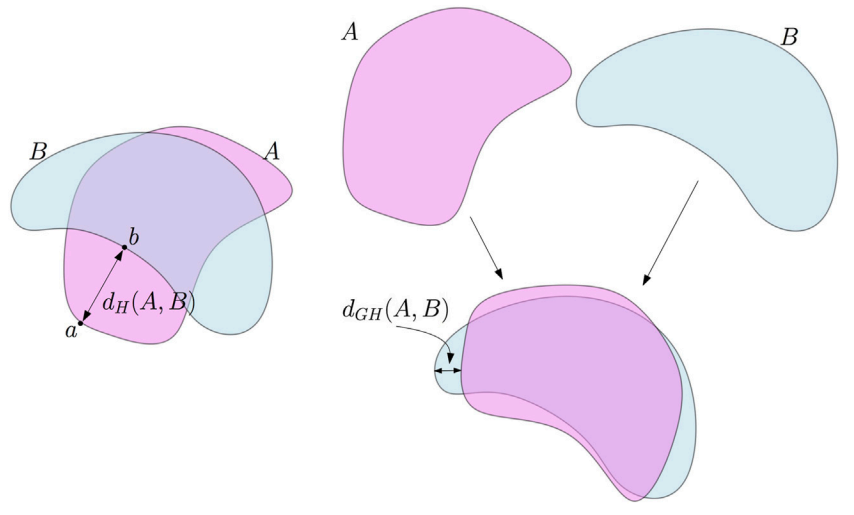
\includegraphics[width=0.85\linewidth]{./figures/Figura1_c1.png}
    \caption{
        Izquierda: la distancia de Hausdorff entre dos subconjuntos $A$ y $B$ en el plano. en este ejemplo,
        $d_{H}\left(A, B\right)$ es la distancia entre el punto $a$ en $A$ que es el m\'as lejano a $B$ y
        su vecino m\'as cercano $b$ en $B$. Derecha: la distancia de Gromov-Hausdorff entre $A$ y $B$. $A$
        puede ser rotado para reducir su distancia de Hausdorff a $B$. As\'i, $d_{GH}\left(A, B\right) \leq
        d_{H}\left(A, B\right)$.
    }
    \label{fig:Figura 1}
    \vspace{15pt}
\end{figure}

Usaremos la distancia de Gromov-Hausdorff m\'as adelante para el estudio de las propiedades de estabilidad
de los diagramas de persistencia.

Conectar pares de puntos de datos cercanos mediante aristas lleva a la noci\'on est\'andar de una gr\'afica
simple de la cual la conectividad de los datos puede ser analizada usando, por ejemplo, algoritmos de
agrupamiento. Para ir m\'as all\'a de la conectividad, una idea central en el ATD es construir nociones
equivalentes a las gr\'aficas simples pero de dimensi\'on m\'as alta, utilizando no s\'olo pares sino
$\left(k + 1\right)$-tuplas de puntos de datos cercanos. El resultado son objetos llamados complejos
simpliciales, los cuales nos ayudan a identificar nuevas caracter\'isticas topol\'ogicas tales como ciclos,
huecos, y sus correspondientes de dimensiones superiores.

\section*{Complejos Simpliciales Geom\'etricos y Abstractos}

Los complejos simplicales pueden considerarse como gr\'aficas generalizadas a dimensiones superiores.
Son objetos matem\'aticos que son de naturaleza topol\'ogica y combinatoria a la vez, una propiedad que
los hace particularmente \'utiles para el ATD.

Dado un conjunto $\mathbb{X} = \left\{x_{0}, \dots, x_{k}\right\}\subset\mathbb{R}^{d}$ con $k + 1$
puntos af\'inmente independientes, el simplejo $k$-dimensional
$\sigma = \left[x_{0}, \dots, x_{k}\right]$ generado por $\mathbb{X}$ es la envolvente convexa de
$\mathbb{X}$. Los puntos de $\mathbb{X}$ son llamados v\'ertices de $\sigma$, y los simplejos generados
por los subconjuntos de $\mathbb{X}$ son llamados caras de $\sigma$. Un complejo simplicial geom\'etrico
$K$ en $\mathbb{R}^{d}$ es una colecci\'on de simplejos que cumplen lo siguiente:

\begin{enumerate}[label=\roman*)]
    \item Cualquier cara de un simplejo de $K$ es un simplejo de $K$ y,
    
    \item La intersecci\'on de cualesquiera dos simplejos de $K$ es el conjunto vac\'io o una cara com\'un
    de ambos simplejos.
    
\end{enumerate}

La uni\'on de los simplejos de $K$ es un subconjunto de $\mathbb{R}^{d}$ llamado el espacio subyacente
de $K$ que hereda la topolog\'ia de $\mathbb{R}^{d}$. As\'i, $K$ puede ser visto como un espacio
topol\'ogico a trav\'es de su espacio subyacente. Es de notar que una vez que se conocen los v\'ertices,
$K$ se encuentra completamente caracterizado por la descripci\'on combinatoria de una colecci\'on de
simplejos que satisfacen ciertas reglas de incidencia.

Dado un conjunto $V$, un complejo simplicial abstracto con un conjunto de v\'ertices $V$ es un conjunto
$\tilde{K}$, de subconjuntos finitos de $V$ tales que los elementos de $V$ pertenecen a $\tilde{K}$ y
que para cualquier $\sigma \in \tilde{K}$, cualquier subconjunto de $\sigma$ pertenece a $\tilde{K}$.
Los elementos de $\tilde{K}$ son llamados las caras o los simplejos de $\tilde{K}$. La dimensi\'on
de un simplejo abstracto es su cardinalidad menos 1 y la dimensi\'on de $\tilde{K}$ es la mayor de las
dimensiones de sus simplejos. Es de notar que los complejos simpliciales de dimensi\'on $1$
son gr\'aficas.

La descripci\'on combinatoria de cualquier complejo simplicial geom\'etrico $K$ da lugar a un complejo
simplicial abstracto $\tilde{K}$. El inverso tambi\'en es cierto; siempre es posible asociar con un
complejo simplical abstracto $\tilde{K}$ un cierto espacio topol\'ogico $|\tilde{K}|$
tal que si $K$ es un complejo simplicial geom\'etrico cuya descripci\'on combinatoria es la misma
que la de $\tilde{K}$, entonces el espacio subyacente de $K$ es homeomorfo a $|\tilde{K}|$.
Dicha $K$ es llamada una realizaci\'on geom\'etrica de $\tilde{K}$. Como consecuencia de esto,
los complejos simpliciales abstractos pueden ser vistos como espacios topol\'ogicos y los complejos
simpliciales geom\'etricos pueden ser vistos como realizaciones geom\'etricas de la estructura combinatoria
subyacente. As\'i, se puede considerar a los complejos simpliciales como objetos combinatorios que se
ajustan bien a c\'alculos computacionales efectivos y a su vez como espacios topol\'ogicos de los cuales se pueden
inferir propiedades topol\'ogicas.

\section*{Construcci\'on de Complejos Simpliciales a partir de Datos}

Dado un conjunto de datos, o m\'as generalmente, un espacio m\'etrico o topol\'ogico, existen varias
maneras de construir complejos simpliciales. Esta es una presentaci\'on de algunos ejemplos cl\'asicos
que son usados con frecuencia en la pr\'actica.

Comenzando con una extensi\'on inmediata de la noci\'on de una gr\'afica, Sup\'ongase que
tenemos un conjunto de puntos $\mathbb{X}$ en un espacio m\'etrico $\left(M, \rho\right)$ y un n\'umero
real $\alpha \geq 0$. El complejo de Vietoris-Rips $Rips_{\alpha}\left(\mathbb{X}\right)$ es el conjunto
de simplejos $\left[x_{0}, \dots, x_{k}\right]$ tal que
$\rho_{\mathbb{X}}\left(x_{i}, x_{j}\right)\leq\alpha$ para todo
$\left(i, j\right)$, ver Figura \ref{fig:Figura 2}. De aqu\'i vemos que el complejo de
Vietoris-Rips es efectivamente
un complejo simplicial abstracto. Aunque, en general, incluso cuando $\mathbb{X}$ es un subconjunto
finito de $\mathbb{R}^{d}$, $Rips_{a}\left(\mathbb{X}\right)$ no admite una realizaci\'on geom\'etrica en
$\mathbb{R}^{d}$; en particular, puede ser de una dimensi\'on mayor a $d$, por ejemplo, si se tienen $d+2$
puntos en $R^{d}$ que cumplen $\rho_{\mathbb{X}}\left(x_{i},x_{j}\right)\leq\alpha$ para todo
$\left(i,j\right)$, entonces $Rips_{a}\left(\mathbb{X}\right)$ es de dimensi\'on $d+1$, podemos ver un
caso similar en el tetraedro formado en el complejo derecho de la Figura \ref{fig:Figura 2}.

Estrechamente relacionado al complejo de Vietoris-Rips est\'a el complejo de
\v Cech $Cech_{a}\left(\mathbb{X}\right)$ el cual se define como el conjunto de simplejos
$\left[x_{0}, \dots, x_{k}\right]$ tales que las $k + 1$ bolas cerradas $B\left(x_{i},\alpha\right)$
tienen intersecci\'on no vac\'ia, ver Figura \ref{fig:Figura 2}. Estos dos complejos estan relacionados por

\begin{equation*}
    Rips_{\alpha}\left(\mathbb{X}\right)\subseteq
    Cech_{\alpha}\left(\mathbb{X}\right)\subseteq
    Rips_{2\alpha}\left(\mathbb{X}\right)
\end{equation*}

\noindent y que si $\mathbb{X}\subset\mathbb{R}^{d}$, entonces $Cech_{\alpha}\left(\mathbb{X}\right)$ y
$Rips_{2\alpha}\left(\mathbb{X}\right)$ tienen el mismo esqueleto $1$-dimensional, esto es, comparten el
mismo conjunto de v\'ertices y aristas.

\begin{figure}[ht]
    \centering
    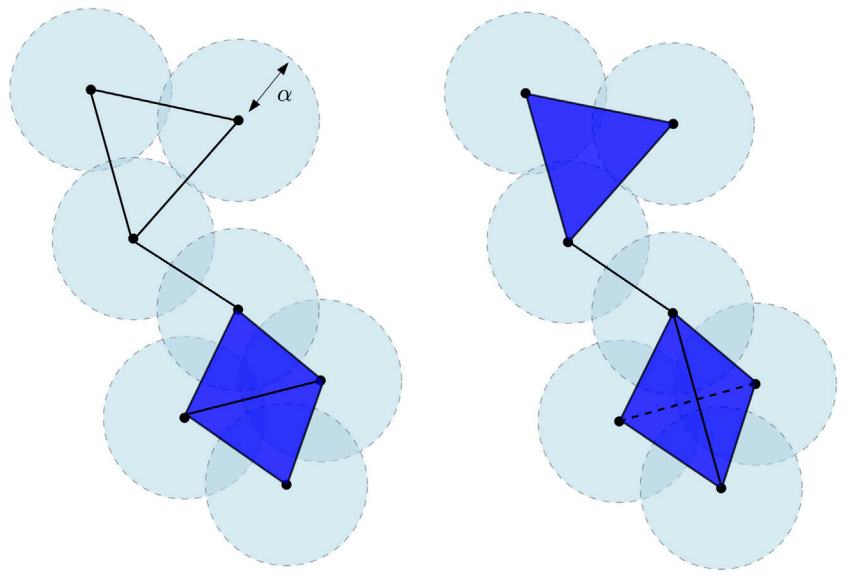
\includegraphics[width=0.85\linewidth]{./figures/Figura2_c1.png}
    \caption{
        El complejo de \v Cech, $Cech_{\alpha}\left(\mathbb{X}\right)$ (izquierda) y el de Vietoris-Rips
        $Rips_{2\alpha}\left(\mathbb{X}\right)$ (derecha) en una nube finita de puntos en
        $\mathbb{R}^{2}$. La parte inferior de $Cech_{\alpha}\left(\mathbb{X}\right)$ es la uni\'on de
        dos tri\'angulos adyacentes, mientras que la parte inferior de
        $Rips_{2\alpha}\left(\mathbb{X}\right)$ es el tetraedro generado por los cuatro v\'ertices
        y todas sus caras. La dimensi\'on del complejo de \v Cech es $2$. La dimensi\'on del complejo
        de Vietoris-Rips es $3$. Es de notar que el complejo de Vietoris-Rips, en este caso, no puede ser inmerso en $\mathbb{R}^{2}$.
    }
    \label{fig:Figura 2}
    \vspace{15pt}
\end{figure}

\section*{El Teorema del Nervio}

El complejo de \v Cech es un caso particular de una familia de complejos asociados con cubiertas. Dada
una cubierta $\mathcal{U}=\left(U_{i}\right)_{i\in I}$ de $\mathbb{M}$, conjunto de puntos en
$\mathbb{R}^{d}$, es decir, una familia de conjuntos $U_{i}$ tales que
$\mathbb{M}=\cup_{i\in I}U_{i}$, el nervio de $\mathcal{U}$ es el complejo simplicial
abstracto $C\left(\mathcal{U}\right)$ cuyos v\'ertices son los $U_{i}$'s y que cumple

\begin{equation*}
    \sigma = \left[U_{i_{0}}, \dots, U_{i_{k}}\right] \in C\left(\mathcal{U}\right)
    \text{ si y s\'olo si } \cap_{j=0}^{k}U_{i_{j}}\neq\varnothing.
\end{equation*}

Dada una cubierta de un conjunto de datos, donde cada conjunto de la cubierta es, por ejemplo, una
agrupaci\'on de los puntos de los datos que tienen ciertas propiedades en com\'un,
su nervio proporciona una descripci\'on combinatoria, compacta y global, de las relaciones
entre estos conjuntos a trav\'es de sus patrones de intersecci\'on. Ver Figura (\ref{fig:Figura 3}).

\begin{figure}[ht]
    \centering
    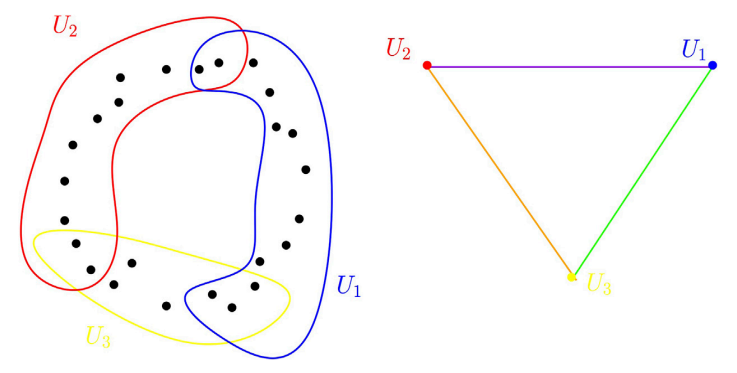
\includegraphics[width=0.85\linewidth]{./figures/Figura3.png}
    \caption{
        Nube de puntos muestreada en el plano y una cubierta de conjuntos abiertos para esta
        nube (izquierda). El nervio de esta cubierta es un tri\'agulo (derecha).
        Los v\'ertices corresponden a uno de los conjuntos de la cubierta mientras que
        las aristas corresponden a una de las
        intersecciones no vac\'ias entre dos conjuntos de la cubierta.
    }
    \label{fig:Figura 3}
    \vspace{15pt}
\end{figure}

Un teorema fundamental en topolog\'ia algebraica se encarga de relacionar, bajo ciertas condiciones, la
topolog\'ia del nervio de una cubierta con la topolog\'ia de la uni\'on de los conjuntos
de dicha cubierta. Es necesario introducir algunas nociones adicionales para ser
formales a la hora de enunciar este
resultado conocido como el teorema del nervio.

Dos espacios topol\'ogicos, $X$ y $Y$, usualmente son considerados iguales desde un punto de vista
topol\'ogico si son homeomorfos, esto es, si existen dos funciones, biyectivas y continuas,
$f:X\rightarrow Y$ y $g:Y\rightarrow X$ tales que $f\circ g$ y $g\circ f$ son las funciones
identidad de $Y$ y $X$, respectivamente. En muchas ocasiones, pedir que $X$ y $Y$ sean
homeomorfos resulta ser una condici\'on demasiado fuerte para asegurar que $X$ y $Y$
compartan propiedades topol\'ogicas de inter\'es para el ATD.
Dos funciones continuas $f_{0}, f_{1}:X\rightarrow Y$ se dicen ser homot\'opicas
si existe una funci\'on continua $H:X\times\left[0, 1\right]\rightarrow Y$ tal que para
cualquier $x\in X$, $H\left(x, 0\right) = f_{0}\left(x\right)$ y $H\left(x, 1\right) = g\left(x\right)$.
Los espacios $X$ y $Y$ se dicen ser homot\'opicamente equivalentes si existen
dos funciones, $f:X\rightarrow Y$ y $g:Y\rightarrow X$, tales que $f\circ g$ y $g\circ f$ son
homot\'opicas a la func\'on identidad de $Y$ y $X$, respectivamente.
Las funciones $f$ y $g$ son llamadas homot\'opicamente equivalentes. La noci\'on de
equivalencia homot\'opica es m\'as d\'ebil que la de homeomorfismo; si $X$ y $Y$ son homeomorfos, entonces
son homot\'opicamente equivalentes, pero el rec\'iproco no es cierto. Sin embargo, espacios que son
homot\'opicamente equivalentes a\'un comparten muchos invariantes topol\'ogicos, como la conexidad por
caminos, los grupos de homotop\'ia y, en particular, tienen la misma homolog\'ia.

Un espacio se dice ser contra\'ible si es homot\'opicamente equivalente a un punto. Las bolas, y en
general los conjuntos convexos en $\mathbb{R}^{d}$, son ejemplos b\'asicos de espacios contra\'ibles.
Las cubiertas abiertas, para las cuales se tiene que todos sus elementos e intersecciones son
contra\'ibles, tienen la siguiente propiedad.

\begin{teorema}[Teorema del Nervio]\label{teoNervio}
    Sea $\mathcal{U} = \left(U_{i}\right)_{i\in I}$ una
    cubierta abierta de un espacio topol\'ogico $X$ tal que la intesecci\'on
    de cualquier subcolecci\'on de los $U_{i}$'s es contra\'ible o vac\'ia.
    Entonces, $X$ y el nervio $C\left(\mathcal{U}\right)$ son
    homot\'opicamente equivalentes.
\end{teorema}

Es f\'acil verificar que subconjuntos convexos de espacios euclidianos son contra\'ibles. Como
consecuencia, si $\mathcal{U} = \left(U_{i}\right)_{i\in I}$ es una colecci\'on de subconjuntos convexos
de $\mathbb{R}^{d}$, entonces $C\left(\mathcal{U}\right)$ y $\cup_{i\in I}U_{i}$ son homot\'opicamente
equivalentes. En particular, si $\mathbb{X}$ es un conjunto de puntos en $\mathbb{R}^{d}$, entonces el
complejo de \v Cech $Cech_{\alpha}\left(\mathbb{X}\right)$ es homot\'opicamente equivalente a la uni\'on
de bolas $\cup_{x\in\mathbb{X}}B\left(x, \alpha\right)$.

El teorema del nervio juega un papel fundamental en el ATD; proporciona una manera de codificar la
topolog\'ia de espacios continuos en estructuras combinatorias abstractas que se ajustan con facilidad
al dise\~{n}o de estructuras de datos y algoritmos efectivos.
\chapter{Utilizando Cubiertas y Nervios para el An\'alisis de Datos Exploratorio y Visualizaci\'on: El
Algoritmo Mapper.}

Usar el nervio de cubiertas como una manera de visualizar y explorar datos es una idea natural que fue
propuesta para el ATD en el estudio por Singh et al. \cite{Singh2007}, dando lugar al algoritmo Mapper.

\begin{definicion}
    Sea $f:\mathbb{X}\rightarrow\mathbb{R}^{d}$, $d\geq1$, una funci\'on continua y sea
    $\mathcal{U} = \left(U_{i}\right)_{i\in I}$ una cubierta de $\mathbb{R}^{d}$. laL cubierta pull-back
    de $\mathbb{X}$ inducida por $\left(f, \mathcal{U}\right)$ es la colecci\'on de conjuntos abiertos
    $\left(f^{-1}\left(U_{i}\right)\right)_{i\in I}$. El pull-back refinado es una colecci\'on de
    componentes conexas de los abiertos $f^{-1}\left(U_{i}\right)$, $i\in I$.
\end{definicion}

La idea del algoritmo Mapper es, dado un conjunto de datos $\mathbb{X}$ y una funci\'on
$f:\mathbb{X}\rightarrow\mathbb{R}^{d}$, sintetizar $\mathbb{X}$ a trav\'es del nervio
del pull-back refinado de una cubierta $\mathcal{U}$ de $f\left(\mathbb{X}\right)$. Para cubiertas bien
escogidas $\mathcal{U}$, este nervio es una gr\'afica que encapsula de manera conveniente el detalle de los
datos y los vuelve f\'aciles de visualizar (Ver Figura \ref{fig:Figura 4}).

El algoritmo de Mapper es muy sencillo; pero este recalca las diferentes elecciones que son dejadas al
usuario y que discutiremos a continuaci\'on.

\begin{itemize}
    \item \textbf{Entrada:} Un conjunto de datos $\mathbb{X}$ con una m\'etrica o medida de disimilaridad
    entre los puntos asociados a los datos, una funci\'on $f:\mathbb{X}\rightarrow\mathbb{R}$
    (o bien, $f:\mathbb{X}\rightarrow\mathbb{R}^{d}$), y una cubierta $\mathcal{U}$
    de $f\left(\mathbb{X}\right)$.
    Para cada $U\in\mathcal{U}$, descomponer $f^{-1}\left(U\right)$ en agrupaciones
    $C_{U,1}, \dots, C_{U,k_{U}}$. Calcular el nervio de la cubierta de $X$ definido por los
    $C_{U,1}, \dots, C_{U,k_{U}}$, $U\in\mathcal{U}$.
    
    \item \textbf{Salida:} Un complejo simplicial; el nervio que incluye un v\'ertice $v_{U,i}$ por cada
    $C_{U,i}$ y una arista entre cada uno de los v\'ertices $v_{U,i}$ y $v_{U',j}$ que cumplan
    $C_{U,i}\cap C_{U',j} \neq \varnothing$.
    
\end{itemize}

\newpage

\begin{figure}[ht]
    \centering
    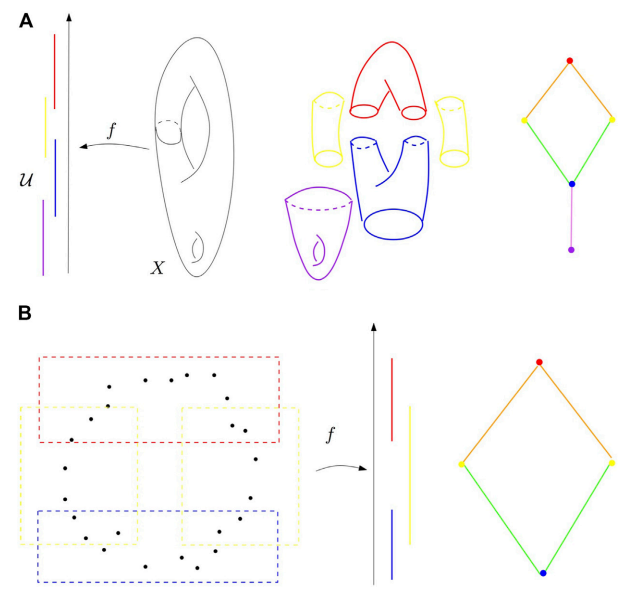
\includegraphics[width=0.85\linewidth]{./figures/Figura4.png}
    \caption{
        (A) Cubierta pull-back refinada de la funci\'on altura sobre una superficie en $\mathbb{R}^{3}$.
        (B) Algoritmo de Mapper en una nube de puntos muestreada alrededor de un c\'irculo y la
        funci\'on altura.
    }
    \label{fig:Figura 4}
    \vspace{15pt}
\end{figure}

\section*{La Elecci\'on de $f$}

La elecci\'on de la funci\'on $f$, a veces llamada la funci\'on filtro o lente, depende fuertemente de las
propiedades de los datos que uno pretende resaltar. Las siguientes son algunas de las m\'as encontradas en
la literatura:

\begin{itemize}
    \item Estimadores de densidad: El complejo Mapper puede ser \'util para entender la estructura y
    conexidad de \'areas de alta densidad.
    
    \item Coordenadas de an\'alisis de componentes principales (coordenadas PCA) o funciones coordenadas
    obtenidas de una t\'ecnica de reducci\'on de dimensionalidad no lineal (NLDR), eigenfunciones de
    laplacianos de gr\'aficas pueden ayudar a revelar y entender parte de la ambig\"uedad en el uso
    de reducciones de dimensionalidad no lineales.
    
    \item La funci\'on de centralidad $f\left(x\right) = \Sigma_{y\in\mathbb{X}}d\left(x,y\right)$ y la
    funci\'on de excentricidad $f\left(x\right) = \max_{y\in\mathbb{X}}d\left(x,y\right)$ a veces resultan
    ser buenas elecciones que no requieren de ning\'un conocimiento espec\'ifico acerca de los datos.
    
    \item Para datos muestreados sobre estructuras filamentarias de dimensi\'on uno, la funci\'on
    distancia a un punto dado permite recuperar la topolog\'ia subyacente de las estructuras filamentarias
    \cite{Chazal2015d}.
    
\end{itemize}

\section*{La Elecci\'on de la Cubierta $\mathcal{U}$}

Cuando $f$ es una funci\'on de valores reales, una elecci\'on est\'andar de $\mathcal{U}$
es un conjunto de intervalos espaciados regularmente y del mismo largo, $r>0$, cubriendo al conjunto
$f\left(\mathbb{X}\right)$. El n\'umero real $r$ es a veces llamado la resoluci\'on de
la cubierta, y el porcentaje $g$ de sobreposici\'on entre dos
intervalos consecutivos es llamado la ganancia de la cubierta.
N\'otese que si la ganancia $g$ es escogida menor a $50\%$, entonces cada punto de la linea real es
cubierto por, a lo m\'as, $2$ conjuntos abiertos de $\mathcal{U}$, y el nervio
resultante es una gr\'afica. Es importante notar que la salida de Mapper es muy
sensible a la elecci\'on de $\mathcal{U}$, y cambios
peque\~{n}os en la resoluci\'on o ganancia puede afectar de manera significativa al resultado, volviendo el
m\'etodo muy inestable. Una estrategia cl\'asica consiste en explorar un rango de par\'ametros y
seleccionar aquellos que sean m\'as informativos desde el punto de vista del usuario.

\section*{La Elecci\'on del Agrupamiento}

El algoritmo Mapper requiere el agrupamiento de la preimagen de conjuntos abiertos $U\in\mathcal{U}$.
Existen dos estrategias para realizar este agrupamiento. La primera consiste en aplicar, a cada
$U\in\mathcal{U}$, un algoritmo de agrupamiento, escogido por el usuario, a la preimagen de
$f^{-1}\left(U\right)$. La segunda, m\'as global, consiste en construir una gr\'afica sobre el
conjunto de datos $\mathbb{X}$, por ejemplo, una gr\'afica k-NN o una $\epsilon$-gr\'afica y, para cada
$U\in\mathcal{U}$, tomar las componentes conexas de la subgr\'afica con el conjunto de v\'ertices
$f^{-1}\left(U\right)$.

\section*{Aspectos Teor\'eticos y Estad\'isticos del Algoritmo Mapper}

Basados en los resultados de estabilidad y la estructura de Mapper propuestos en el estudio por
Carri\`ere y Oudot (2017) \cite{Carriere2017}, se han realizado avances en direcci\'on a
una versi\'on de Mapper estad\'isticamente bien fundamentada en el estudio por Carri\`ere et al. (2018)
\cite{Carriere2018}. De aqu\'i destaca que la convergencia de Mapper depende tanto del muestreo de los
datos como de la regularidad de la funci\'on filtro. M\'as aun, estrategias de submuestreo pueden ser
usadas para seleccionar un complejo en una filtraci\'on de Rips a una escala conveniente, as\'i como la
resoluci\'on y la ganancia para definir la gr\'afica Mapper. El caso para filtros estoc\'asticos y
multivariados tambi\'en ha sido estudiado por Carri\`ere y Michel (2019) \cite{Carriere2019}.
Una descripci\'on alternativa de la convergencia probabil\'istica de Mapper, en t\'erminos de la
categorificaci\'on, fue propuesta en el estudio por Brown et al. (2020) \cite{Brown2020}. Otros
acercamientos tambi\'en fueron propuestos para estudiar y lidiar con la inestabilidad del algoritmo
Mapper en los trabajos de Dey et al. (2016) \cite{Dey2016}, Dey et al. (2017) \cite{Dey2017}.

\section*{An\'alisis de Datos con Mapper}

Como una herramienta del an\'alisis de datos, Mapper se ha utilizado con \'exito para tareas de
agrupamiento y selecci\'on de atributos. La idea es identificar estructuras
espec\'ificas en la gr\'afica (o complejo) Mapper, en particular, lazos.
Estas estructuras son usadas para identificar
c\'umulos interesantes o seleccionar atributos que puedan diferenciar los datos en estas estructuras de
manera apropiada. Aplicaciones en datos reales ilustrando estas t\'ecnicas pueden ser encontradas en,
por ejemplo, los estudios por Carri\`ere y Rabad\'an (2020) \cite{Carriere2020}, Lum et al. (2013)
\cite{Lum2013}, Yao et al. (2009) \cite{Yao2009}.
\chapter{Reconstrucci\'on Geom\'etrica e Inferencia Homol\'ogica}

Otra forma de construir cubiertas y usar sus nervios para exhibir la estructura topol\'ogica de los datos
es considerar la uni\'on de bolas centradas en los puntos de los datos. En esta secci\'on suponemos que
$\mathbb{X}_n = \left\{x_0, \dots, x_n\right\}$ es un subconjunto de $\mathbb{R}^{d}$, muestrado de manera
i. i. d. de acuerdo con la medida de probabilidad $\mu$ con soporte compacto $M\subset\mathbb{R}^{d}$. La
estrategia general para inferir informaci\'on topol\'ogica acerca de $M$ a trav\'es de $\mu$ consiste en
dos pasos:

\begin{enumerate}
    \item Se cubre $\mathbb{X}_{n}$ con una uni\'on de bolas de radio fijo con centros en las $x_{i}$'s.
    Bajo algunas condiciones de regularidad en $M$, se puede relacionar la topolog\'ia de esta uni\'on de
    bolas con la de $M$.
    
    \item Desde un una perspectiva pr\'actica y algor\'itmica, las cualidades topol\'ogicas de $M$ son
    inferidas del nervio de la uni\'on de las bolas, utilizando el teorema del nervio.
    
\end{enumerate}

De esta manera, es posible comparar espacios a trav\'es de equivalencias isot\'opicas, una noci\'on m\'as
fuerte que la de homeomorfismo: $X\subseteq\mathbb{X}^{d}$ y $Y\subseteq\mathbb{X}^{d}$ se dicen ser
(ambientalmente) isot\'opicos si existe una familia continua de homeomorfismos
$H: \left[0, 1\right]\times\mathbb{R}^{d}\rightarrow\mathbb{R}^{d}$, $H$ continua, tal que, para cualquier
$t\in\left[0, 1\right]$, $H_{t} = H\left(t, \cdot\right):\mathbb{R}^{d}\rightarrow\mathbb{R}^{d}$ es un
homeomorfismo, $H_{0}$ es el mapeo identidad en $\mathbb{R}^{d}$, y $H_{1}\left(X\right)=Y$.
Es claro que, si $X$ y $Y$ son isot\'opicos, entonces son homeomorfos. El rec\'iproco no es cierto:
un c\'irculo anudado y uno desanudado en $\mathbb{R}^{3}$ son homeomorfos pero no isot\'opicos.

\section*{Funciones DL y Reconstrucci\'on}

Dado un suconjunto compacto $K\subset\mathbb{R}^{d}$ y un n\'umero real no negativo $r$, la uni\'on de
bolas de radio $r$ centradas en $K$, $K^{r} = \cup_{x\in K}B\left(x, r\right)$, llamado el
$r$-cubrimiento de $K$, es el conjunto de $r$-subnivel de la distancia
$d_{K}:\mathbb{R}^{d}\rightarrow\mathbb{R}$ definida por
$d_{K}\left(x\right) = \inf_{y\in K}\left\|x-y\right\|$; es decir,
$K^{r} = d^{-1}_{k}\left(\left[0, r\right]\right)$. Esto nos permite utilizar propiedades diferenciales
de funciones distancia y nos ayuda a comparar la topolog\'ia de los cubrimientos de conjuntos compactos
 que est\'en cercas el uno del otro con respecto a la distancia de Hausdorff.
 
\begin{definicion}
    (Distancia de Hausdorff en $\mathbb{R}^{3}$). La distancia de Hausdorff entre dos subconjuntos compactos
    $K$, $K'$ de $\mathbb{R}^{d}$ esta definida como
    \begin{equation*}
        d_{H}\left(K, K'\right) = \left\|d_{K}-d_{K'}\right\|_{\infty} =
        \inf_{x\in\mathbb{R}^{d}}\left|d_{K}\left(x\right)-d_{K'}\left(x\right)\right|
    \end{equation*}
\end{definicion}
 
Aqu\'i, los conjuntos compactos son el conjunto de datos $\mathbb{X}_{n}$ y el soporte $M$ de la
medida $\mu$. Cuando $M$ es una subvariedad compacta suave, bajo ciertas condiciones sobre
$d_{H}\left(\mathbb{X}_{n}, M\right)$, para alg\'un $r$ bien escogido, las coberturas de
$\mathbb{X}_{n}$ son homot\'opicamente equivalentes a $M$, Chazal y Lieutier (2008) \cite{Chazal2008},
Niyogi et al. (2008) \cite{Niyogi2008} (Ver Figura \ref{fig:Figura 5}). Estos resultados se extienden
a clases m\'as grandes de conjuntos compactos y llevan a resultados fuertes sobre inferencia de los
tipos de isotop\'ias de las coberturas de $M$, Chazal et al. (2009c) \cite{Chazal2009c},
Chazal et al. (2009d)\cite{Chazal2009d}. Tambi\'en llevan a resultados en la estimaci\'on de otras
cantidades geom\'etricas y diferenciales tales como normales, Chazal et al. (2009c) \cite{Chazal2009c},
curvaturas Chazal et al. (2009e) \cite{Chazal2009e}, o medidas de frontera,
Chazal et al. (2010) \cite{Chazal2010} bajo ciertas condiciones en la distancia de Hausdorff entre la
forma subyacente y los datos muestrales.
 
Estos resultados dependen de la $1$-semiconcavidad del cuadrado de la funci\'on distancia $d_{K}^{2}$,
esto es, la convexidad de la funci\'on $x\rightarrow\left\|x\right\|^{2}-d_{K}^{2}\left(x\right)$,
definida de a continuaci\'on.
 
\begin{definicion}
    Una funci\'on $\phi:\mathbb{R}^{d}\rightarrow\mathbb{R}_{+}$ es DL (distance-like) si es propia (la
    preimagen de cualquier conjunto compacto en $\mathbb{R}$ bajo $\phi$ es un compacto en
    $\mathbb{R}^{d}$) y $x\rightarrow\left\|x\right\|^{2}-\phi^{2}\left(x\right)$ es convexa.
\end{definicion}
 
Gracias a su semiconcavidad, una funci\'on DL $\phi$ tiene un gradiente
$\nabla\phi:\mathbb{R}^{d}\rightarrow\mathbb{R}^{d}$ bien definido, pero no continuo, que puede ser
integrado en un flujo continuo (Petrunin, 2007 \cite{Petrunin2007}) que permite rastrear la evoluci\'on
de la topolog\'ia de sus subniveles y compararla a una de los subniveles de funciones DL cercanas.
 
\begin{definicion}
    Sea $\phi$ una funci\'on DL y sea $\phi^{r}=\phi^{-1}\left(\left[0,r\right]\right)$ el $r$-subnivel
    de $\phi$.
    
    \begin{itemize}
        \item Un punto $x\in\mathbb{R}^{d}$ es llamado $\alpha$-cr\'itico si
        $\left\|\nabla_{x}\phi\right\|\leq\alpha$. El valor $r=\phi\left(x\right)$ correspondiente,
        tambi\'en es llamado $\alpha$-cr\'itico.
        
        \item El tama\~{n}o del atributo d\'ebil de $\phi$ en $r$ es el m\'inimo $r>0$ tal que $\phi$
        no tiene ning\'un valor cr\'itico entre $r$ y $r+r'$. Lo denotamos por
        $\mathrm{wfs}_{\phi}\left(r\right)$ (weak feature size). Para cualquier $0<\alpha<1$, el 
        $\alpha$-alcance de $\phi$ es el m\'aximo $r$ tal que $\phi^{-1}\left(\left(0,r\right]\right)$
        no contiene ning\'un punto $\alpha$-cr\'itico.
        
    \end{itemize}
\end{definicion}
 
El tama\~{n}o del atributo d\'ebil $\mathrm{wfs}_{\phi}\left(r\right)$ (respecto al $\alpha$-alcance)
mide la regularidad de $\phi$ sobre sus $r$-niveles (respecto al $O$-nivel). Cuando $\phi=d_{K}$ es
la funci\'on distancia a un conjunto compacto $K\subset\mathbb{R}^{d}$, el $1$-alcance coincide con el
alcance cl\'asico de la teor\'ia de la medida gem\'etrica, Federer (1959) \cite{Federer1959}. Su
estimaci\'on desde muestras aleatorias fue estudiada en Aamari et al. (2019) \cite{Aamari2019}. Una
propiedad importante de una funci\'on DL $\phi$ es que la topolog\'ia de sus subniveles $\phi^{r}$
s\'olo puede cambiar cuando $r$ cruza un valor $0$-cr\'itico.

\begin{lema}
    (Lema de isotop\'ia). Sea $\phi$ una funci\'on DL y $r_{1}<r_{2}$ dos n\'umeros positivos tales que
    $\phi$ no tiene puntos $0$-cr\'iticos, esto es, puntos $x$ tales que $\nabla\phi\left(x\right)=0$,
    en el subconjunto $\phi^{-1}\left(\left[r_{1},r_{2}\right]\right)$. Entonces todos los subniveles
    $\phi^{-1}\left(\left[0,r\right]\right)$ son isot\'opicos para $r\in\left[r_{1},r_{2}\right]$.
\end{lema}

\begin{figure}[ht]
    \centering
    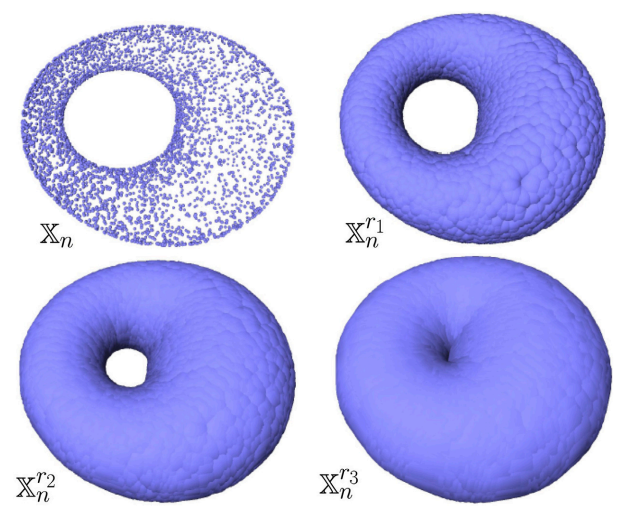
\includegraphics[width=0.85\linewidth]{./figures/Figura5.png}
    \caption{
        Ejemplo de una nube de puntos $\mathbb{X}_{n}$ muestreada en la
        superficie de un toro en $\mathbb{R}^{3}$ y sus coberturas para
        diferentes valores del radio $r_{1}<r_{2}<r_{3}$. Para valores
        bien escogidos del radio (por ejemplo $r_{1}$ y $r_{2}$), las
        coberturas son homot\'opicamente equivalentes al toro.
    }
    \label{fig:Figura 5}
    \vspace{15pt}
\end{figure}

Como consecuencia inmediata del lema de isotop\'ia, todos los subniveles de $\phi$ entre $r$ y
$r + \mathrm{wfs}_{\phi}\left(r\right)$ tienen la misma topolog\'ia. Ahora, el siguiente teorema de
Chazal et al. \cite{Chazal2011b}, proporciona una conexi\'on entre la topolog\'ia de los subniveles
de funciones DL cercanas.

\newpage

\begin{teorema}[Teorema de reconstrucci\'on]\label{teoRecon}
    Sean $\phi$, $\psi$ dos funciones DL, tales que
    $\left\|\phi-\psi\right\|_{\infty}\leq\epsilon$, con $\alpha$-alcance
    $\mathrm{reach}_{\alpha}\left(\phi\right)\geq R$ para algunos $\epsilon$ y $\alpha$ positivos.
    Entonces, para todo $r\in\left[4\epsilon/\alpha^{2}, R-3\epsilon\right]$ y cada
    $\eta\in\left(0, R\right)$ los subniveles $\psi^{r}$ y $\phi^{\eta}$ son homot\'opicamente
    equivalentes si:
    
    \begin{equation*}
        \epsilon\leq\frac{R}{5+4/\alpha^{2}}
    \end{equation*}
\end{teorema}

Bajo condiciones similares pero ligeramente m\'as t\'ecnicas, el teorema de reconstrucci\'on puede ser
extendido para probar que los subniveles son homeomorfos e incluso isot\'opicos
(Chazal et al., 2009 \cite{Chazal2009c}; Chazal et al., 2008 \cite{Chazal2008}).

Consideremos una vez m\'as $\phi = d_{M}$ y $\psi = d_{\mathbb{X}_{n}}$ las funciones distancia
al soporte de $M$ de la medida $\mu$ y al conjunto de puntos asociados a los datos $\mathbb{X}_{n}$,
la condici\'on $\mathrm{wfs}_{\alpha}\left(d_{M}\right)\geq R$ puede ser interpretada como una
condici\'on de regularidad sobre $M$\footnote{Por ejemplo, si $M$ es una subvariedad compacta suave,
el $0$-alcance $\mathrm{reach}_{0}\left(\phi\right)$ siempre es positivo se le llama el alcance de
$M$ Federer (1959) \cite{Federer1959}}. El teorema de reconstrucci\'on junto con el teorema del nervio
nos indican que para ciertos valores de $r$, $\eta$ y los $\eta$-cobertura son homot\'opicamente
equivalentes al nervio de la uni\'on de las bolas de radio $r$ centradas en $\mathbb{X}_{n}$, es decir,
el complejo de \v Cech $Cech_{r}\left(\mathbb{X}_{n}\right)$.

Desde un punto de vista estad\'istico, la principal ventaja de estos resultados sobre la distancia de
Hausdorff es que el problema de estimaci\'on de cantidades topol\'ogicas se transforma en una serie
de preguntas acerca de el soporte de ciertas medidas, las cuales han sido ampliamente estudiadas.

\section{Inferencia Homol\'ogica}

Los resultados anteriores proporcionan una estructura matem\'atica bien fundamentada para inferir la
topolog\'ia de las formas de un complejo simplicial construido sobre una muestra finita que sirve como
aproximaci\'on. Sin embargo, desde una perspectiva m\'as pr\'actica, aparecen dos problemas. Primero, el
teorema de reconstrucci\'on requiere de regularidad a trav\'es de la condici\'on del $\alpha$-alcance
que a veces no puede ser garantizada, adem\'as de la elecci\'on del radio $r$ que se debe realizar para
construir el complejo de \v Cech $Cech_{r}\left(\mathbb{X}_{n}\right)$. Segundo,
$Cech_{r}\left(\mathbb{X}_{n}\right)$ brinda una fiel descripci\'on topol\'ogica de los datos a trav\'es
de un complejo simplicial que normalmente no es adecuado para un procesamiento de datos adicional. Es
conveniente tener descriptores topol\'ogicos que sean f\'aciles de manejar, en particular descriptores
num\'ericos, que pueden ser calculados desde el complejo simplicial de manera sencilla. Este segundo
problema se resuelve al considerar la homolg\'ia del complejo simplicial en cuesti\'on,
tema que se desarrollara a continuaci\'on, por otra parte, el primer problema sera resuelto
en la siguiente cap\'itulo con la introducci\'on a la homolog\'ia persistente.

\subsubsection*{Homolog\'ia}

La homolog\'ia es un concepto cl\'asico en la topolog\'ia algebraica, brinda una herramienta poderosa
para formalizar y manejar la noci\'on de caracter\'isticas topol\'ogicas de un espacio topol\'ogico o
un complejo simplicial de manera algebraica. Para cualquier dimensi\'on $k$, los ``hoyos''
$k$-dimensionales son representados por un espacio vectorial $H_{k}$, cuya dimeni\'on es el n\'umero
de dichas propiedades. Por ejemplo, el grupo de homolog\'ia $0$-dimensional $H_{0}$ representa las
componentes conexas del complejo, el grupo de homolog\'ia $1$-dimensional $H_{1}$ representa los lazos
de dimensi\'on uno, el grupo de homolog\'ia $2$-dimensional $H_{2}$ representa las cavidades de
de dimensi\'on dos, y as\'i sucesivamente.

Para evitar dificultades y sutilezas t\'ecnicas, restringimos esta introducci\'on a la homolog\'ia al
m\'inimo necesario para continuar con nuestro programa. En particular, nos restringimos al caso
donde la homolog\'ia tiene coeficientes en $\mathbb{Z}_{2}$, esto es, el campo con dos elementos,
$0$ y $1$, tales que $1 + 1 = 0$, que tiene una interpretaci\'on geom\'etrica m\'as intuitiva. No
obstante, todas las nociones y resultados presentados aqu\'i se extienden de manera natural a la
homolog\'ia con coeficientes en cualquier campo. Referimos al lector al estudio por Hatcher
(2001) \cite{Hatcher2001} para una introducci\'on completa a la homolog\'ia y al estudio por Ghrist
(2017) \cite{Ghrist2017} para una introducci\'on concisa y reciente a la topolog\'ia algebraica
aplicada y sus conexiones con el an\'alisis de datos.

Sea $K$ un complejo simplicial (finito) y $k$ un entero no-negativo. El espacio de las $k$-cadenas en
$K$, $C_{k}\left(K\right)$ es el conjunto cuyos elementos son las sumas formales (finitas) de los
$k$-simplices de $K$. M\'as precisamente, si $\left\{\sigma_{1},\dots,\sigma_{p}\right\}$ es el
conjunto de los $k$-simplices de $K$, entonces cualquier $k$-cadena puede ser escrita como:

\begin{equation*}
    c = \sum_{i=0}^{p}\epsilon_{i}\sigma_{i} \text{ con } \epsilon_{i}\in\mathbb{Z}_{2} 
\end{equation*}

\begin{figure}[ht]
    \centering
    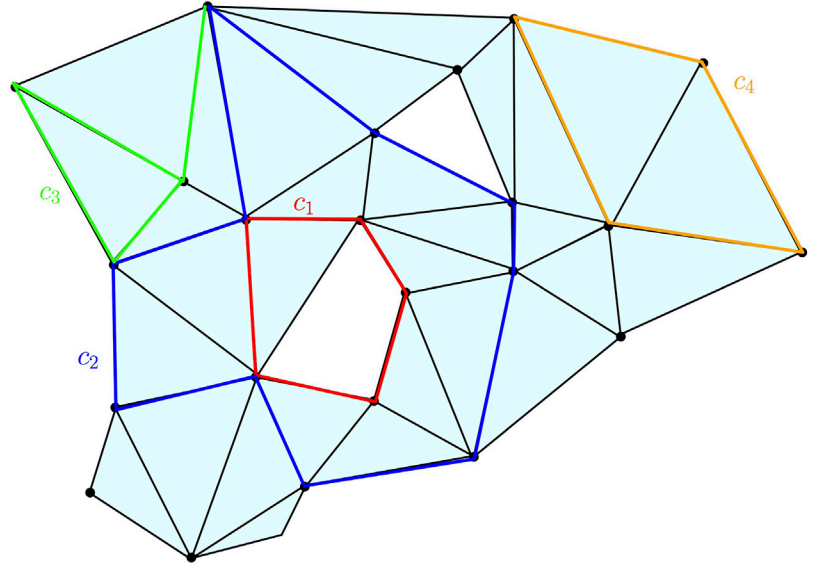
\includegraphics[width=0.85\linewidth]{./figures/Figura6.png}
    \caption{
        Algunos ejemplos de cadenas, ciclos y fronteras en un complejo $K$ de dos dimensiones:
        $c_{1}$, $c_{2}$ y $c_{4}$ son $1$-ciclos; $c_{3}$ es una $1$-cadena pero no un $1$-ciclo;
        $c_{4}$ es una $1$-frontera, la frontera de la $2$-cadena obtenida de la suma de los
        tri\'angulos rodeados por $c_{4}$. Los ciclos $c_{1}$ y $c_{2}$ generan el mismo elemento en
        $H_{1}\left(K\right)$ ya que su diferencia es la $2$-cadena representada por la uni\'on de
        tri\'angulos que rodean la uni\'on de $c_{1}$ y $c_{2}$.
    }
    \label{fig:Figura 6}
    \vspace{15pt}
\end{figure}

Si $c'=\sum_{i=1}^{p}\epsilon_{i}'\sigma_{i}$ es otra $k$-cadena y $\lambda\in\mathbb{Z}_{2}$,
la suma $c+c'$ esta definida como $c+c'=\sum_{i=1}^{p}\left(\epsilon_{i}+\epsilon_{i}'\right)\sigma_{i}$
y el producto $\lambda\cdot c$ esta definido como
$\lambda\cdot c = \sum_{i=1}^{p}\left(\lambda\cdot\epsilon_{i}\right)\sigma_{i}$, convirtiendo a
$C_{k}\left(K\right)$ en un espacio vectorial con coeficientes en $\mathbb{Z}_{2}$. Ya que estamos
considerando los coeficientes en $\mathbb{Z}_{2}$, geom\'etricamente, una $k$-cadena puede ser vista como
una colecci\'on finita de $k$-simplices y la sumas de dos $k$-cadenas como la diferencia sim\'etrica
de las colecciones correspondientes\footnote{Recordemos que la diferencia sim\'etrica entre dos conjuntos
$A$ y $B$ es el conjunto $A\Delta B = \left(A\\B\right)\cup\left(B\\A\right)$}.

La frontera de un $k$-simplejo $\sigma = \left[v_{k},\dots,v_{k}\right]$ es la $\left(k-1\right)$-cadena

\begin{equation*}
    \partial_{k}\left(\sigma\right) = \sum_{i=0}^{k}\left(-1\right)
    \left[v_{0},\dots,\hat{v}_{i},\dots,v_{k}\right]
\end{equation*}

\noindent donde $\left[v_{0},\dots,\hat{v}_{i},\dots,v_{k}\right]$ es el $\left(k-1\right)$-simplejo
generado por todos los v\'ertices a excepci\'on de $v_{i}$\footnote{Ya que estamos considerando
los coeficientes en $\mathbb{Z}_{2}$, se tiene que $-1=1$ y por lo tanto $\left(-1\right)^{i}=1$
para cualquier $i$.}. Dado que los $k$-simplejos forman una base de $C_{k}\left(K\right)$,
$\partial_{k}$ se extiende como una funci\'on lineal de $C_{k}\left(K\right)$ a $C_{k-1}\left(K\right)$
llamado el operador frontera. El kernel de $\partial_{k}$ denotado por: $Z_{k}\left(K\right)=
\left\{c\in C_{k}\left(K\right):\partial_{k}\left(c\right)=0\right\}$ es llamado el espacio de
$k$-ciclos de $K$, y la imagen de $\partial_{k+1}$ denotada por: $B_{k}\left(K\right)=
\left\{c\in C_{k}\left(K\right): \exists c' \in C_{k+1}\left(K\right),
\partial_{k+1}\left(c'\right)=c\right\}$ es llamada el espacio de $k$-fronteras de $K$.

\begin{figure}[ht]
    \centering
    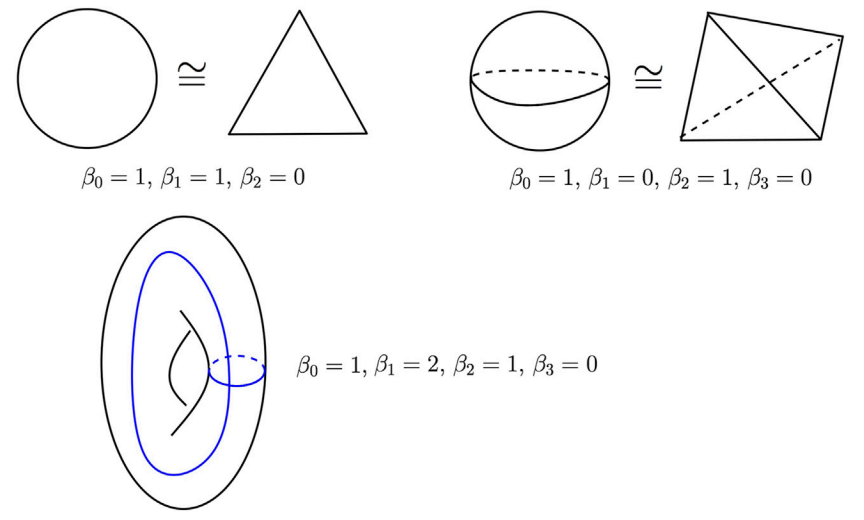
\includegraphics[width=0.85\linewidth]{./figures/Figura7.png}
    \caption{
        N\'umeros de Betti en el c\'irculo, la esfera de dimensi\'on dos y el toro de dimensi\'on dos.
        Las curvas azules en el toro representan dos ciclos independientes cuya clase de homolog\'ia
        es una base para el grupo de homolog\'ia de dimensi\'on uno.
    }
    \label{fig:Figura 7}
    \vspace{15pt}
\end{figure}

\newpage

El operador frontera satisface la siguiente propiedad fundamental:

\begin{equation*}
    \partial_{k+1}\circ\partial_{k+1}\equiv 0 \text{ para cualquier } k\geq 1.
\end{equation*}

\noindent en otras palabras, cualquier $k$-frontera es un $k$-ciclo, esto es,
$B_{k}\left(K\right)\subseteq Z_{k}\left(K\right)\subseteq C_{k}\left(K\right)$. Estas nociones son
ilustradas en la Figura \ref{fig:Figura 6}.

\begin{definicion}
    (grupo de homolog\'ia simplicial y n\'umeros de Betti). El $k$-\'esimo grupo de homolog\'ia
    (simplicial) de $K$ es el espacio cociente
    
    \begin{equation*}
        H_{k}\left(K\right)=Z_{k}\left(K\right)/B_{k}\left(K\right).
    \end{equation*}
    El $k$-\'esimo n\'umero de Betti de $K$ es la dimensi\'on $\beta_{k}\left(K\right)=
    \mathrm{dim}H_{k}\left(K\right)$ del espacio $H_{k}\left(K\right)$.
\end{definicion}

La Figura \ref{fig:Figura 7} muestra los n\'umeros de Betti de algunos espacios sencillos. Dos ciclos,
$c, c' \in Z_{k}\left(K\right)$, se dicen ser hom\'ologos si difieren por una frontera, esto es, si
existe una $\left(k+1\right)$-cadena $d$ tal que $c'=c+\partial_{k+1}\left(d\right)$. Dichos ciclos dan
lugar al mismo elemento de $H_{k}$. En otras palabras, los elementos de $H_{k}\left(K\right)$ son clases
de equivalencia de ciclos hom\'ologos.

Los grupos de homolog\'ia simplicial y los n\'umeros de Betti son invariantes topologicas; si $K$, $K'$
son dos complejos simpliciales tales que sus realizaciones geom\'etricas son homot\'opicamente
equivalentes, entonces sus grupos de homolog\'ia son isomorfos y sus n\'umeros de Betti son iguales.

La homolog\'ia singular es otra noci\'on de homolog\'ia que nos permite considerar una mayor variedad de
espacios topol\'ogicos. Esta definida para cualquier espacio topol\'ogico $X$ de manera similar a la
homolog\'ia simplicial, excepto que el concepto de simplejo, es reemplazado por por el de simplejo
singular, que consiste en una funci\'on continua $\sigma: \Delta_{k}\rightarrow X$ donde $\Delta_{k}$
es el simplejo est\'andar de dimensi\'on $k$. El espacio de las $k$-cadenas es el espacio
vectorial generado por los simplejos singulares $k$-dimensionales, y la frontera de un simplejo $\sigma$
esta definida como la suma (alternante) de la restricci\'on de $\sigma$ a las caras $(k-1)$-dimensionales
de $\Delta_{k}$. Algo importante acerca de la homolog\'ia singular es hecho de que esta coincide con
la homolog\'ia simplicial cuando $X$ es homeomorfo a la realizaci\'on gem\'etrica de un complejo
simplicial. Esto nos permite hablar acerca de la homolog\'ia de un espacio topol\'ogico o un complejo
simplical, sin tener que especificar si nos referimos a la homolog\'ia singular o simplicial.

Observemos que si $f:X\rightarrow Y$ es una funci\'on continua, entonces para cualquier simplejo singular
$\sigma:\Delta_{k}\rightarrow X$ en $X$, se tiene que $f\circ\sigma:\Delta_{k}\rightarrow Y$ es un
simplejo singular en $Y$, de aqu\'i, deducimos que funciones continuas entre espacios topol\'ogicos
inducen homomorfismos entre sus grupos de homolog\'ia. En particular, si $f$ es una equivalencia
homot\'opica, entonces se induce un isomorfismo entre $H_{k}\left(X\right)$ y $H_{k}\left(Y\right)$ para
cualquier $k$ entero no-negativo. Por ejemplo, sea $X\subset \mathbb{R}^{d}$ cualquier conjunto de puntos
y $r>0$, se sigue del teorema del nervio que la $r$-cobertura $X^{r}$ y el complejo de \v Cech
$Cech_{r}\left(X\right)$ tienen grupos de homolog\'ia isomorfos y los mismos n\'umeros de Betti.

%Nuevos comandos

Adem\'as de esto, tenemos como consecuencia del teorema de reconstrucci\'on \ref{teoRecon} el siguiente
resultado que nos auxilia en la estimaci\'on de n\'umeros de Betti.

\begin{teorema}
    Sea $M \subset \mathbb{R}^{d}$ un conjunto compacto con alcance,
    $\mathrm{reach}_{\alpha}\cpar{d_{M}}\geq R > 0$ para alg\'un $\alpha\in\cpar{0, 1}$ y sea $\mathbb{X}$
    un conjunto finito de puntos tales que:
    \begin{equation*}
        d_{H}\cpar{M, \mathbb{R}}=\epsilon < \frac{R}{5+4/\alpha^{2}}.
    \end{equation*}
    Entonces, para cada $r\in\ccorch{4\epsilon/\alpha^{2}, R-3\epsilon}$ y cada $\eta\in\cpar{0, R}$,
    los n\'umeros de Betti de $Cech_{r}\cpar{\mathbb{X}}$ y $M^{\eta}$ son iguales.
    
    En particular, si $M$ es una subvariedad suave de $\mathbb{R}^{d}$ de dimensi\'on $m\in\mathbb{Z}$,
    entonces $\beta_{k}\cpar{Cech_{r}\cpar{\mathbb{R}}}=\beta_{k}\cpar{M}$ para cualquier $k=0, \dots, m$.
\end{teorema}

Desde una perspectiva m\'as pragm\'atica, este resultado nos genera tres problemas: primero, la
suposici\'on de regularidad acerca del $\alpha$-alcance de $M$ puede ser demasiado restrictiva; segundo,
el c\'alculo del nervio de la uni\'on de bolas requiere de m\'etodos para probar que la uni\'on finita de
bolas sea no-vac\'ia; tercero, la estimaci\'on de n\'umeros de Betti recae en la elecci\'on del
par\'ametro $r$.

Para solucionar los problemas anteriores, Chazal y Oudot (2008) \cite{Chazaloudot2008} establecieron el
siguiente resultado que ofrece la soluci\'on a los primeros dos problemas.

\begin{teorema}
    Sea $\mathbb{M}\subseteq\mathbb{R}^{d}$ un conjunto compacto tal que $\mathrm{wfs}\cpar{M}=
    \mathrm{wfs}_{d_{M}}\cpar{0}\geq R>0$ y sea $\mathbb{X}$ un conjunto de puntos finito tal que
    $d_{H}\cpar{M,\mathbb{X}}=\epsilon <\frac{1}{9}\mathrm{wfs}\cpar{M}$. Entonces para cualquier
    $r\in \ccorch{2\epsilon, \frac{1}{4}\cpar{\mathrm{wfs}\cpar{M}-\epsilon}}$ y cualquier
    $\eta\in\cpar{0,R}$,
    \begin{equation*}
        \beta_{k}\cpar{X^{\eta}} = \mathrm{rk}\cpar{H_{k}\cpar{Rips_{r}\cpar{\mathbb{X}}}}
        \rightarrow H_{k}\cpar{Rips_{4r}\cpar{\mathbb{X}}}
    \end{equation*}
    donde $\mathrm{rk}\cpar{H_{k}\cpar{Rips_{r}\cpar{\mathbb{X}}}}
    \rightarrow H_{k}\cpar{Rips_{4r}\cpar{\mathbb{X}}}$ denota el rango de del homomorfismo inducido
    por la inclusi\'on can\'onica (continua)
    $Rips_{r}\cpar{\mathbb{X}}\hookrightarrow Rips_{4r}\cpar{\mathbb{X}}$.
\end{teorema}

Aunque este resultado deja abierta la elecci\'on del par\'ametro $r$, en el estudio realizado por
Chazal y Oudot (2008) \cite{Chazaloudot2008} se provee una descripci\'on de una estrategia multiescala
que ayuda a identificar las escalas relevantes en las cuales se puede aplicar el teorema anterior.

\newpage

\section{Aspectos estad\'isticos de la inferencia homol\'ogica}

De acuerdo a los resultados de estabilidad presentados en la secci\'on anterior, un acercamiento
estad\'istico a la inferencia topol\'ogica se relaciona fuertemente al problema de estimaci\'on de
soportes de distribuciones y estimaciones de conjuntos nivel bajo la m\'etrica de Hausdorff.
Afortunadamente se cuenta con una variedad de metodos y resultados que nos atudan a estimar el soporte de
una distribuci\'on. Por ejemplo, el estimador de Devroye y Wise
(Devroye y Wise 1980 \cite{DevroyeWise1980}) definido en una muestra $\mathbb{X}_{n}$ es tambi\'en una
cobertura  particular de $\mathbb{X}_{n}$. La tasa de convergencia de $\mathbb{X}_{n}$ y el estimador
de Devroye y Wise al soporte de la distribuci\'on para la distancia de Hausdorff fueron estudiados por
Cuevas y Rodriguez-Casal (2004) \cite{CuevasRodriguezCasal2004} en $\mathbb{R}^{d}$. Recientemente, las
tasas de convergencia minimax de estimaci\'on de variedades bajo la metrica de Hausdorff, particularmente
relevantes para la inferencia topol\'ogica, fueron estudiadas por Genovese et al. (2012)
\cite{Genovese2012}. Tambi\'en existe literatura acerca de la estimacion de los conjuntos de nivel en
varias m\'etricas (vease, por ejemplo, Cadre, 2006 \cite{Cadre2006}; Polonik, 1995 \cite{Polonik1995};
Tsybakov, 1997 \cite{Tsybakov1997}) y, particularmente, para la m\'etrica de Hausdorff Chen et al.
(2017) \cite{Chen2017}. Todos estos trabajos acerca de la estimaci\'on de soportes y conjuntos nivel,
dan lugar al an\'alisis estad\'istico de procesos de inferecia topol\'ogica.

En el estudio por Nigoyi et al (2008) \cite{Niyogi2008}, se muestra que el tipo de homotop\'ia de
variedades Riemannianas con alcance mayor que cierta constante puede ser recuperado con una
alta probabilidad de las coberturas de una muestra en (o bien, cerca) de la variedad en cuesti\'on.
Este articulo fue probablemente el primer intento de considerar la inferencia topol\'ogica en t\'erminos
de probabilidad. El estudio por Nigoyi et al.\cite{Niyogi2008} derivo de un argumento de contracci\'on de
retracto y utiliz\'o cotas estrechas sobre el n\'umero de cobertura de la variedad para controlar
la distancia de Hausdorff entre la variedad y la nube de puntos observada. La inferencia homol\'ogica
en el caso de ruido presente, esto es, en el sentido de que la distribuci\'on de la observaci\'on se
concentra alrededor de la variedad, tambi\'en fue estudiado por Nigoyi et al. (2008) \cite{Niyogi2008},
Nigoyi et al. (2011) \cite{Niyogi2008}. La suposici\'on de que el objeto geom\'etrico es una variedad
Riemanniana suave solo es usada en el art\'iculo para controlar la distancia de Hausdorff entre la
muestra y la variedad y no es realmente necesaria para la ``parte topol\'ogica'' del resultado, el cual
es similar a aquellos en los estudios por Chazal et al. (2009) \cite{Chazal2009d}, Chazal y Lieutier
(2008) \cite{Chazal2008} en el entorno particular de las variedades Riemannianas. Empezando por el
resultado del estudio por Nigoyi et al. (2008) \cite{Niyogi2008}, las tasas de convergencia minimax
del tipo de homolog\'ia han sido estudiadas por Balakrishnan et al, (2012) \cite{Balakrishnan2012}
bajo varios modelos de variedades Riemannianas con alcance m\'as grande que cierta constante. En contraste, no se ha propuesto una versi\'on estad\'istica del trabajo por Chazal et al. (2009)
\cite{Chazal2009d}.

M\'as recientemente, siguiendo las ideas encontradas en Nigoyi et al. (2008) \cite{Niyogi2008},
Bobrowski et al (2014) \cite{Bobrowski2014} se ha propuesto un robusto estimador homol\'ogico para los
conjuntos de nivel de funciones de densidad y regresi\'on, por medio de considerar la inclusi\'on entre
pares anidados de conjuntos de nivel estimados obtenidos mediante un estimador del kernel.

\section{M\'as all\'a de la Distancia de Hausdorff: Distancia a una Medida}

Es bien sabido que los m\'etodos del ATD fallan rotundamente en presencia de puntos aislados, a\~{n}adir
un solo punto asilado al conjunto de datos puede alterar la funci\'on distacia de manera dram\'atica
(ver Figura \ref{fig:Figura 8}). Como respuesta a esto, Chazal et al. (2011) \cite{Chazal2011b}
introdujeron una funci\'on distancia alternativa la cual es resistente ante el ruido, la distancia a una
medida.

Dada una distribuci\'on de probabilidad $P$ en $\mathbb{R}^{d}$ y un par\'ametro real $0\leq U\leq 1$,
la noci\'on de distancia al soporte de $P$ puede ser generalizada como la funci\'on

\begin{equation*}
    \delta_{P,u}:x\in\mathbb{R}^{d}\mapsto\inf{t>0:P\cpar{B\cpar{x,t}}\geq u}
\end{equation*}

donde $B\cpar{x,t}$ es la bola cerrada (Euclideana) con centro en $x$ y radio $t$. Para evitar problemas
de discontinuidad con la funci\'on $P\rightarrow \delta_{P,u}$, la funci\'on distancia a la medida (DAM)
con par\'ametro $m\in\ccorch{0,1}$ y potencia $r\geq 1$ esta definida como

\begin{equation}
    d_{P,m,r}\cpar{x}:
    x\in\mathbb{R}^{d}\mapsto\cpar{\frac{1}{m}\int_{0}^{m}\delta_{P,u}^{r}\cpar{x}\,du}^{\frac{1}{r}}
\end{equation}

\par Una propiedad deseable de las DAM demostrada por Chazal et al. (2011)\cite{Chazal2011b} es la
estabilidad con respecto a las perturbaciones de $P$ en la m\'etrica de Wasserstein, m\'as precisamente,
la funci\'on $P\rightarrow d_{P,m,r}$ es $m^{-\frac{1}{r}}$-Lipschitz, esto es, si $P$ y $\tilde{P}$ son
dos distribuciones de probabilidad en $\mathbb{R}^{d}$, entonces

\begin{equation}
    \cnorm{d_{P,m,r}-d_{\tilde{P},m,r}}_{\infty}\leq m^{-\frac{1}{r}}W_{r}\cpar{P,\tilde{P}}
\end{equation}

donde $W_{r}$ es la distancia de Wasserstein para la m\'etrica Euclidiana en $\mathbb{R}^{d}$, con
exponente $r$\footnote{Ver Villiani (2003)\cite{Villiani2003} para la definici\'on de distancia de
Wasserstein}. Esta propiedad implica que la DAM asociada con distribuciones cercanas en la m\'etrica de
Wasserstein tienen conjuntos subnivel cercanos. M\'as a\'un, cuando $r=2$, la funci\'on
$d_{P,m,2}^{2}$ es semiconcava, lo cual asegura fuertes propiedades de regularidad en la
geometr\'ia de sus subniveles. Usando estas propiedades, Chazal et al. (2011) \cite{Chazal2011b} mostr\'o
que bajo suposiciones generales, si $\tilde{P}$ es una distribuci\'on de probabilidad que aproxima a $P$,
as\'i los conjuntos subnivel de $d_{\tilde{P},m,2}$ proveen una aproximaci\'on topol\'ogicamente
correcta al soporte de $P$.

\par En la pr\'actica, la medida $P$ usualmente solo es conocida a trav\'es de un conjunto finito de
observaciones $\mathbb{X}_{n}=\cllav{X_{1},\dots,x_{n}}$ muestreada desde $P$, dando lugar a la pregunta
de una aproximaci\'on a la DAM. Una idea natural para estimar la DAM desde $\mathbb{X}_{n}$ es utilizar
la medida emp\'irica $P_{n}$ en lugar de $P$ en la definici\'on de la DAM. Esto corresponde al computo
de la distancia à la medida emp\'irica (DAME). Para $m=\frac{k}{n}$, la DAME satisface

\begin{equation*}
    d_{P_{n},k/n,r}^{r}\cpar{x}:=\frac{1}{k}\sum_{j=1}^{k}\cnorm{x-\mathbb{X}_{n}}_{\cpar{j}}^{r}
\end{equation*}

donde $\cnorm{x-\mathbb{X}_{n}}_{\cpar{j}}$ denota la distancia entre $x$ y su $j$-\'esima vecindad
en $\cllav{X_{1},\dots,X_{n}}$. Esta cantidad es f\'acil de calcular en la pr\'actica ya que solo
requiere de distancias entre $x$ y los puntos de la muestra. La convergencia de las DAME a las DAM
ha sido estudiada por Chazal et al. (2017)\cite{Chazal2017} y Chazal et al (2016)\cite{Chazal2016b}.

La introducci\'on de las DAM a motivado trabajos y aplicaciones en diferentes direcciones tales como
el an\'lisis topol\'ogico de datos (Buchet et al., 2015\cite{Buchet2015a}), an\'alisis de trazas GPS
(Chazal et al., 2011 \cite{Chazal2011a}), estimaci\'on de densidad (Biau et al., 2011 \cite{Biau2011}),
pruebas de hip\'otesis (Br\'echeteau, 2019 \cite{Brecheteau2019}), y agrupamiento (Chazal et al., 2013
\cite{Chazal2013b}), solo para nombrar algunos. Tambi\'en se han tomado en consideraci\'on,
aproximaciones, generalizaciones, y variantes de las DAM (Guibas et al., 2013 \cite{Guibas2013};
Phillips et al., 2014 \cite{Phillips2014}; Buchet et al., 2015 \cite{Buchet2015b};
Br\'echeteau y Levrard, 2020 \cite{Brecheteau2020}).

\begin{figure}[ht]
    \centering
    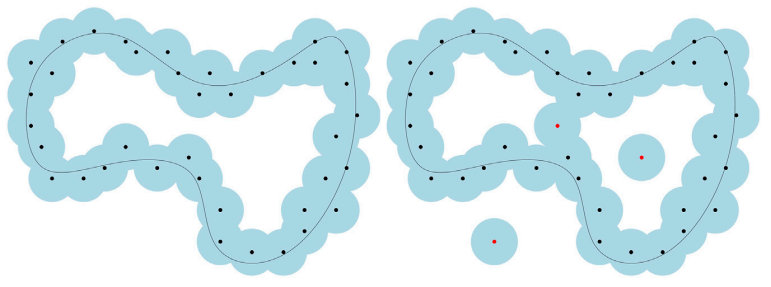
\includegraphics[width=0.85\linewidth]{./figures/Figura8.png}
    \caption{
        Efectos de los puntos aislados en los conjuntos subnivel de las funciones distancia. A\~{n}adir
        unos pocos puntos aislados a la nube puede alterar dram\'aticamente la funci\'on distancia y
        la topolog\'ia de sus coberturas.
    }
    \label{fig:Figura 8}
    \vspace{15pt}
\end{figure}
\chapter{Homolog\'ia Persistente}

La homolog\'ia persistente es una herramienta poderosa que es usada para el computo, estudio y codificaci\'on
multiescala de propiedades topol\'ogicas de familias anidadas de complejos simpliciales y espacios
topol\'ogicos. No solo provee algoritmos eficientes para calcular los n\'umeros de Betti de cada complejo
en las familias consideradas, como se requiere para la inferencia homol\'ogica cubierta en la secci\'on
anterior, sino que tambi\'en codifica la evoluci\'on de los grupos de homolog\'ia de los
complejos anidados a trav\'es de las escalas. Ideas y resultados preliminares que culminan en la
teor\'ia de la homolog\'ia persistente pueden ser encontrados desde antes del siglo XXI, en particular
en los trabajos de Barannikov (1994) \cite{Barannikov1994}, Frosini (1992) \cite{Frosini1992},
Robins (1999) \cite{Robins1999}; pero su desarrollo en su forma moderna se concreto en los trabajos
de Edelsbrunner et al. (2002) \cite{Edelsbrunner2002} y Zomorodian y Carlsson (2005)
\cite{Zomorodian2005}.

\section{Filtraciones}

Una filtraci\'on de un complejo simplicial $K$ es una familia anidada de subcomplejos
$\cpar{K_{r}}_{r\in t}$, donde $T\subseteq\mathbb{R}$, tal que para cualquier
$r, r' \in T$, si $r\leq r'$ entonces $K_{r}\subseteq K_{r'}$ y $K = \bigcup_{r\in T}K_{r}$.
El subconjunto $T$ puede ser finito o infinito. En general, una filtraci\'on de un espacio
topol\'ogico $\mathbb{M}$ es una familia anidada de subespacios $\cpar{M_{r}}_{r\in T}$,
donde $T\subseteq\mathbb{R}$, tal que para cualquier $r, r' \in T$,
si $r\leq r'$ entonces $M_{r}\subseteq M_{r'}$ y $M = \bigcup_{r\in T}M_{r}$. Por ejemplo, si
$f: \mathbb{M}\rightarrow\mathbb{R}$ es una funci\'on, entonces la familia
$M_{r} = f^{-1}\cpar{\left(-\infty, r\right]}$, $r\in\mathbb{R}$ define una filtraci\'on llamada la
filtraci\'on del conjunto subnivel de $f$.

En la pr\'actica, el par\'ametro $r\in T$ suele ser interpretado como un par\'ametro de escala, y las
filtraciones com\'unmente usadas en el ATD suelen pertenecer a uno de los siguientes dos tipos.

\section*{Filtraciones Sobre Datos}

Dado un subconjunto $\mathbb{X}$ de un espacio m\'etrico compacto $\cpar{M,\rho}$, las familias de
complejos de Vietoris-Rips $\cpar{Rips_{r}\cpar{\mathbb{X}}}_{r\in\mathbb{R}}$ y los complejos de \v Cech
$\cpar{Cech_{r}\cpar{\mathbb{X}}}_{r\in\mathbb{R}}$ son filtraciones\footnote{Aqu\'i consideramos
$Rips_{r}\cpar{\mathbb{X}} = Cech_{r}\cpar{\mathbb{X}} = \varnothing$, si $r<0$}. Aqu\'i, el par\'ametro
$r$ puede ser interpretado como la resoluci\'on con la que se considera el conjunto de datos $\mathbb{X}$.
Por ejemplo, si $\mathbb{X}$, es una nube de puntos en $\mathbb{R}^{d}$, gracias al teorema del nervio,
la filtraci\'on $\cpar{Cech_{r}\cpar{\mathbb{X}}}_{r\in\mathbb{X}}$ codifica la topolog\'ia de todo la
familia de uniones de bolas $\mathbb{X}^{r} = \cup_{x\in\mathbb{X}}B\cpar{x,r}$, cuando $0<r<\infty$.
Como la noci\'on de filtraci\'on es algo flexible, se han considerado muchas otras filtraciones en la
literatura para ser construidas sobre los datos, como el complejo testigo popularizado en el ATD por
De Silva y Carlsson (2004)\cite{DeSilva2004}, las filtraciones de Rips con peso Buchet et al.
(2015)\cite{Buchet2015b}, o las filtraciones DTM Anai et al. (2019)\cite{Anai2019} que nos permiten
trabajar con conjuntos de datos con ruido o con datos at\'ipicos.

\section*{Filtraciones de Conjuntos Subnivel}

Definir funciones en los v\'ertices de un complejo simplicial da lugar a otro importante ejemplo de
filtraci\'on: sea $K$ el complejo simplicial con el conjunto de v\'ertices $V$ y
$f:V\rightarrow\mathbb{R}$. Entonces $f$ puede ser extendida a todos los simplices de $K$ definiendo
$f\cpar{\ccorch{v_{0},\dots,v_{k}}} = \max\cllav{f\cpar{v_{i}}: i=1,\dots,k}$ para cualquier simplejo
$\sigma = \ccorch{v_{0},\dots,v_{k}}\in K$ y la familia de subcomplejos,
$K_{r}=\cllav{\sigma\in K:f\cpar{\sigma}\leq r}$, define una filtraci\'on llamada la filtraci'on del
conjunto subnivel de $f$. La filtraci\'on del conjunto sobre-nivel de $f$ se define de manera similar.

En la pr\'actica, incluso si el \'indice del conjunto es infinito, todas las filtraciones consideradas
son construidas en conjuntos finitos y son, en si, finitas. Por ejemplo, cuando $\mathbb{X}$ es finito,
el complejo de Vietoris-Rips $Rips_{r}\cpar{\mathbb{X}}$ cambia solo en un numero finito de \'indices,
$r$. Esto nos permite manejarlos de manera sencilla desde una perspectiva algebraica.

\section{Algunos Ejemplos}\label{sec: 4.2}

Dada una filtraci\'on $\mathit{Filt} = \cpar{F_{r}}_{r\in T}$ de un complejo simplicial o un espacio
topol\'ogico, la homolog\'ia de $F_{r}$ cambia cuando $r$ incrementa; pueden aparecen nuevos componentes
conexos y algunos ya existentes pueden unirse, aros y cavidades pueden formarse o llenarse, etc. La
homolog\'ia persistente registra estos cambios, identifica las propiedades que aparecen y asocia un
tiempo de vida a cada una. La informaci\'on resultante se codifica como un conjunto de intervalos llamado
c\'odigo de barras, o bien, como un conjunto de puntos en $\mathbb{R}^{2}$ donde la coordenada de
cada punto es el punto de inicio y final de cada intervalo correspondiente.

Antes de dar una definici\'on formal, ilustraremos el concepto de homolog\'ia persistente con unos
ejemplos.

% IDE Change, change to hard-wrapping per sentence instead of hard-wrapping per max number of char.

\section*{Ejemplo 1}

Sea $f:\ccorch{0,1}\rightarrow\mathbb{R}$ la funci\'on de la Figura \ref{fig:Figura 9},
y sea $F_{r} = f^{-1}\cpar{\cpar{-\infty,r}}_{r\in\mathbb{R}}$ la filtraci\'on del conjunto subnivel de $f$.
Todos los conjuntos subnivel de $f$ son o bien vacios o la uni\'on de intervalos,
as\'i que la \'unica informaci\'on topol\'ogica no-trivial que brindan es su homolog\'ia cero dimensional, esto es, su n\'umero de componenetes conexas.
Para $r<a_{1}$, $F_{r}$ es vacio, pero para $r = a_{1}$, aparecen un primer componente conexo en $F_{a_{1}}$.
La homolog\'ia persistente registra $a_{1}$ como la ``fecha de nacimiento'' de una componente conexa la codifica como un intervalo que comienza en $a_{1}$.
Luego, $F_{r}$ permanece conexo hasta que $r$ toma el valor de $a_{2}$ donde una segunda componente conexa aparece.
La homolog\'ia persitente registra esta nueva componente conexa creando un segundo intervalo que comienza en $a_{2}$.
De manera similar, cuando $r$ alcanza el valor de $a_{3}$, una nueva componente conexa aparece y la homolog\'ia persistente crea otro intervalo comenzando en $a_{3}$.
Cuando $r$ alcanza $a_{4}$, las dos componentes creadas en $a_{1}$ y $a_{3}$ se juntan para crear una sola componente conexa.
En este paso, la homolog\'ia persistente sigue la regla de que la componente que muere es la m\'as reciente que ha aparecido en la filtraci\'on;
As\'i, el intervalo que comenz\'o en $a_{3}$ termina en $a_{4}$,
y el intervalo de persistencia que codifica el tiempo de vida de la componente nacida en $a_{3}$ es creado.
Cuando $r$ alcanza $a_{5}$, como en el caso previo la componente nacida en $a_{2}$ muere y se crea el intervalo $\cpar{a_{2},a_{5}}$.
El intervalo creado en $a_{1}$ permanece hasta el final de la filtraci\'on,
dando lugar al intervalo $\cpar{a_{1},a_{6}}$ si la filtraci\'on se detiene en $a_{6}$,
o bien, $\cpar{a_{1},\infty}$ si $r$ tiende a $+\infty$ (en cuyo caso la filtraci\'on se mantiene constante para $r>a_{6}$).
El conjunto de intervalos obtenidos que codifican el tiempo de vida de diferentes caracter\'isticas homol\'ogicas a lo largo de la filtrac\'on es llamado el c\'odigo de barras de persistencia de $f$.
Cada intervalo $\cpar{a,a'}$ puede ser representado en el plano $\mathbb{R}^{2}$ por el punto $\cpar{a,a'}$.
El conjunto de puntos resultante es llamado el diagrama de persistencia de $f$.
Es de notar que la funci\'on puede tener multiples copias del mismo intervalo en su c\'odigo de barras de persitencia.
Como consecuencia, el diagrama de persistencia de $f$ es un multiconjunto donde cada punto tiene una multiplicidad entera asociada.
Finalmente, por razones t\'ecnicas que seran claras m\'as adelante,
se a\~{n}aden al diagrama de persistencia todos los puntos de la diagonal $\Delta = \cllav{\cpar{b,d}: b=d}$ con multiplicidad infinita.

\begin{figure}[ht]
    \centering
    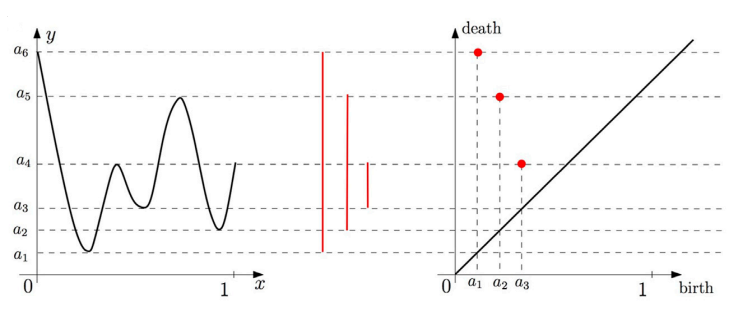
\includegraphics[width=0.85\linewidth]{./figures/Figura9.png}
    \caption{
        El c\'odigo de barras de persistencia y el diagrama de persistencia de la funci\'on
        $f:\ccorch{0,1}\rightarrow\mathbb{R}$.
    }
    \label{fig:Figura 9}
    \vspace{15pt}
\end{figure}

\section*{Ejemplo 2}

Sea $f: M\rightarrow \mathbb{R}$ la funci\'on en la Figura \ref{fig:Figura 10},
donde $M$ es una superficie de dos dimensiones homeomorfa a un toro,
y sea $F_{r} = f^{-1}\cpar{\cpar{-\infty,r}}_{r\in \mathbb{R}}$ la filtraci\'on del conjunto subnivel de $f$.
La homolog\'ia persistente cero dimensional se calcula como en el ejemplo anterior,
lo cual genera las barras rojas en el c\'odigo de barras de persistencia.
En este caso los subniveles tambi\'en almacenan informaci\'on acerca de caracter\'isticas homol\'ogicas uno dimensionales.
Cuando $r$ alcanza la altura $a_{1}$,
los conjuntos subnivel $F_{r}$ que eran homeomorfos a dos discos se vuelven homeomorfos a la uni\'on disjunta de un disco y un \'anulo,
creando un primer ciclo hom\'ologo a $\sigma_{1}$ en la Figura \ref{fig:Figura 10}.
El nacimiento de este uno-ciclo es representado por un intervalo (en azul) que comienza en $a_{1}$.
Similarmente, cuando $r$ alcanza $a_{2}$, un segundo ciclo, hom\'ologo a $\sigma_{2}$, es creado,
dando lugar al comienzo de un nuevo intervalo de persistencia.
Estos dos ciclos nunca son rellenos (abarcan $H_{1}\cpar{M}$) de manera que los intervalos que les corresponden continuan por el resto de la filtraci\'on.
Cuando $r$ alcanza $a_{3}$, un nuevo ciclo es creado, el cual se rellena en $a_{4}$,
lo cual genera el intervalo de persistencia $\cpar{a_{3},a_{4}}$.
Esta vez, la filtraci\'on del conjunto subnivel da lugar a dos c\'odigos de barras,
uno par la homolog\'ia cero dimensional (mostrado en rojo) y otro para la homolog\'ia uno dimensional (mostrado en azul).
Estos dos c\'odigos de barras pueden ser representados de manera equivalente como diagramas en el plano. 

\begin{figure}[ht]
    \centering
    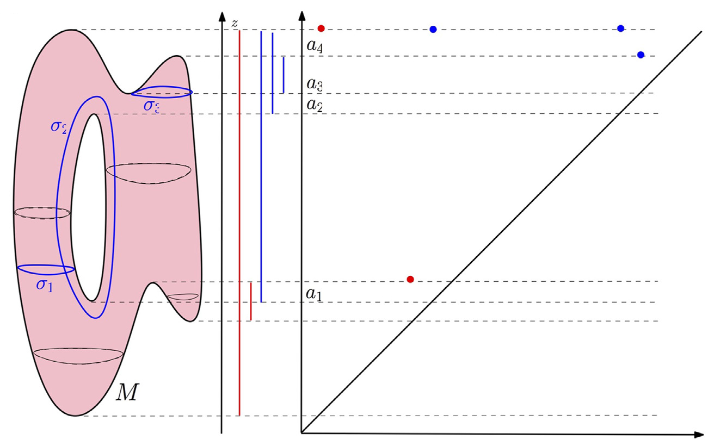
\includegraphics[width=0.85\linewidth]{./figures/Figura10.png}
    \caption{
        El c\'odigo de barras de persistencia y el diagrama de persistencia de la funci\'on altura
        (proyecci\'on en el eje $z$) definida en una superficie en $\mathbb{R}^{3}$.
    }
    \label{fig:Figura 10}
    \vspace{15pt}
\end{figure}

\section*{Ejemplo 3}

En este \'ultimo, consideramos la filtraci\'on dada por la uni\'on de bolas
(que crecen linealmente)
centradas en el conjunto de puntos finitos $C$ en la Figura \ref{fig:Figura 11}.
Notese que esta es la filtraci\'on del conjunto subnivel de la funci\'on distancia a $C$,
y gracias al teorema del nervio,
esta filtraci\'on es homot\'opicamente equivalente a la filtraci\'on de \v Cech construida sobre $C$.
La Figura \ref{fig:Figura 11} muestra varios conjuntos subnivel de la filtraci\'on de la siguiente manera:

\begin{enumerate}[label=\alph*)]
    \item Para radio $r=0$, la uni\'on de bolas se reduce al conjunto de puntos finito inicial,
    cada uno de ellos correspondiendo a una componente conexa;
    se comienza un intervalo por cada una de estas componentes en $r=0$.

    \item Algunas de las bolas comienzan a superponerse,
    resultando en la muerte de algunas de las componentes conexas que se han juntando entre s\'i;
    el diagrama de persistencia registra estas muertes, poniendo fin a los intervalos correspondientes.
    
    \item M\'as componentes conexas se han juntado, dejando una sola componente conexa,
    y as\'i, todos los intervalos asociados a caracter\'isticas cero dimensionales terminan,
    con la excepci\'on de los que corresponden a las componentes restantes;
    dos nuevas caracter\'isticas uno dimensionales han aparecido,
    lo cual resulta en dos nuevos intervalos (en azul) que comienzan en ese valor de $r$.
    
    \item Una de los dos ciclos uno dimensionales se ha rellenado,
    resultando en su muerte en la filtraci\'on y en el fin del intervalo correspondiente.
    
    \item Todas la componenetes uno dimensionales han muerto, dejando un \'unico intervalo rojo en el c\'odigo de barras.
    como en ejemplos anteriores, el c\'odigo de barras puede ser representado como un diagrama de persistencia,
    donde cada intervalo $\cpar{a,b}$ es representa por un punto en $\mathbb{R}^{2}$ de coordenadas correspondientes.
    
\end{enumerate}

Intuitivamente afirmamos que entre m\'as largo sea un intervalo en el c\'odigo de barras,
o bien, equivalentemente,
entre m\'as alejado est\'e un punto de la diagonal en el diagrama correspondiente,
m\'as persistente, y por tanto, relevante, es la propiedad homol\'ogica que le corresponde a trav\'es de la filtraci\'on.
Es de notar tambi\'en que para un radio $r$ dado, el $k$.-\'esimo n\'umero de Betti de la uni\'on de bolas en cuesti\'on,
es igual al n\'umero de intervalos de persistencia correspondiendo a caracter\'isticas homol\'ogicas $k$ dimensionales que contienen a $r$.
As\'i, el diagrama de persistencia puede ser visto como una firma topol\'ogica que codifica la homolo\'gia de la uni\'on de bolas abiertas,
para todos los radios, as\'i como su evoluci\'on a trav\'es de los valores que toma $r$.

\begin{figure}[ht]
    \centering
    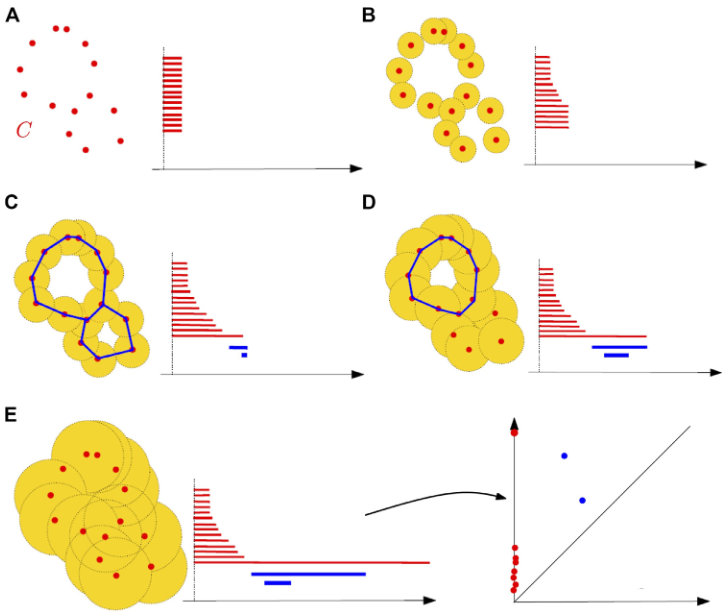
\includegraphics[width=0.85\linewidth]{./figures/Figura11.png}
    % \caption{
    %     Placeholder
    % }
    \label{fig:Figura 11}
    \vspace{15pt}
\end{figure}

\newpage

\section{M\'odulos y Diagramas de Persistencia}

Los diagramas de persistencia pueden ser formalmente definidos de manera puramente algebraica.
No obstante, lo anterior requiere de cuidado,
nos limitaremos a dar nociones b\'asicas dejando de lado sutilesas y dificultades t\'ecnicas.
Una exposici\'on detallada puede encontrarse en el trabajo por Chazal eta al. (2016)\cite{Chazal2016a}.

Sea $\mathit{Filt}=\cpar{F_{r}}_{r\in T}$ una filtraci\'on de un complejo simplicial o un espacio topol\'ogico.
Dado $K$ entero no negativo y considerando los grupos de homolog\'ia $H_{k}\cpar{F_{r}}$,
obtenemos una secuencia de espacios vectoriales donde las inclusiones $F_{r}\subset F_{r'}$, $r\leq r'$
inducen funciones lineales entre $H_{k}\cpar{F_{r}}$ y $H_{k}\cpar{F_{r'}}$.
Dicha secuencia de espacios vectoriales junto con las funciones lineales que los conectan es llamado un m\'odulo de persistencia.

\begin{definicion}
    Un m\'odulo de persistencia $\mathbb{V}$ sobre un subconjunto $T\subset\mathbb{R}$
    es una familia indexada de espacios vectoriales $\cpar{V_{r}|r\in T}$
    y una familia doblemente indexada de funciones lineales $\cpar{v_{s}^{r}:V_{r}\rightarrow V_{s}|r\leq s}$
    la cual satisface la ley de composici\'on $v_{t}^{s}\circ v_{s}^{r}=v_{t}^{r}$ donde $r\leq s\leq t$,
    y donde $v_{r}^{r}$ es la identidad en $V_{r}$.
\end{definicion}

En ocasiones, es posible descomponer un m\'odulo de persistencia en una suma directa de m\'odulos de intervalos $\mathbb{I}_{\cpar{b,d}}$ de la forma

\begin{equation*}
    \dots, \rightarrow 0 \rightarrow \dots, \rightarrow 0 \rightarrow \mathbb{Z}_{2} \rightarrow \dots, \rightarrow \mathbb{Z}_{2} \rightarrow 0 \rightarrow \dots
\end{equation*}

\noindent donde las funciones $\mathbb{Z}_{2}\rightarrow\mathbb{Z}_{2}$ son la identidad y las demas son la funci\'on $0$.
Denotando $b$ y $d$ respectivamente como el \'infimo y el supremo del intervalo de \'indices que corresponden a espacios vectoriales no cero;
dicho m\'odulo puede ser interpretado como una caracter\'istica que aparece en la filtraci\'on en el \'indice $b$ y desaparece en el \'indice $d$.
Cuando un m\'odulo de persistencia $\mathbb{V}$ puede ser descompuesto como una suma directa de m\'odulos de intervalos,
se puede mostrar que esta descomposici\'on es \'unica hasta un reordenamiento de los intervalos
(ver Chazal et al., 2016\cite{Chazal2016a}, Teorema 2.7).
Como consecuencia, el conjunto de intervalos resultantes es independiente de la descomposici\'on de $\mathbb{V}$
y es llamado el c\'odigo de barras de persistencia de $V$.
Como en los ejemplos anteriores,
cada intervalo $\cpar{b,d}$ en el codigo de barras puede ser interpretado como un punto de coordenadas $\cpar{b,d}$ en el plano $\mathbb{R}^{2}$.
La uni\'on disjunta de estos puntos, junto con la diagonal $\Delta =\cllav{x=y}$,
es un multiconjunto llamado el diagrama de persistencia de $\mathbb{V}$.

El siguiente resultado, de (Chazal et al., 2016\cite{Chazal2016a}, Teorema 2.8),
da algunas condiciones necesareas para que sea posible descomponer un m\'odulo de persistencia
en la suma directa de m\'odulos de intervalos.

\begin{teorema}
    Sea $\mathbb{V}$ un m\'odulo de persistencia con \'indices en $T\subset\mathbb{R}$.
    Si $T$ es un conjunto finito o si todos los espacios vectoriales $V_{r}$ son de dimensi\'on finita,
    entonces $\mathbb{V}$ se puede descomponer en una suma directa de m\'odulos de intervalos.
    M\'as a\'un, para cualquier $s,\hspace{2pt}t\in T$, $s\leq t$,
    el n\'umero $\beta_{t}^{s}$ de intervalos que inician antes antes que $s$ y finalizan despues que $t$
    es igual al rango de la funci\'on lineal $v_{t}^{s}$
    y es llamado el n\'umero de Betti \linebreak $\cpar{s, t}$-persistente de la filtraci\'on.
\end{teorema}

Debido a que se satisfacen ambas de las condiciones anteriores para la homolog\'ia persistente de filtraciones de complejos simpliciales finitos,
una consecuencia inmediata de este resultado es que los diagramas de persistencia de dichas filtraciones siempre est\'an bien definidos.

As\'i, es posible mostrar que los diagramas de persistencia pueden ser definidos tan pronto como la siguiente condicion se satisfaga.

\begin{definicion}
    Un m\'odulo de $\mathbb{V}$ con \'indices en $T\subset\mathbb{R}$ es $q$-d\'ocil
    si para todo $r<s$ en $T$, el rango de la funci\'on lineal $v_{s}^{r}:V_{r}\rightarrow V_{s}$ es finito.
\end{definicion}

\begin{teorema}
    Chazal et al. (2009)\cite{Chazal2009a}, Chazal et al. (2016)\cite{Chazal2016a}.
    Si $\mathbb{V}$ es un m\'odulo de persistencia $q$-d\'ocil,
    entonces tiene un diagrama de persistencia bien definido.
    Dicho diagrama de persistencia $\mathrm{dgm}\cpar{\mathbb{V}}$
    es la uni\'on de los puntos de la dioagonal $\Delta$ de $\mathbb{R}^{2}$,
    contados con multiplicidad infinita,
    y un multiconjunto sobre la diagonal en $\mathbb{R}^{2}$ que es localmente finito.
    Aqu\'i, con localmente finito nos referimos a que
    para cualquier rect\'angulo $R$ con lados paralelos a los ejes coordenados que no intersecan a $\delta$,
    el n\'umero de puntos de $\mathrm{dgm}\cpar{\mathbb{V}}$, contados con multiplicidad,
    contenidos en $R$ es finito.
    Adem\'as, a la parte del diagrama hecha de los puntos con segunda coordenada infinita
    es llamada la parte escencial del diagrama.
\end{teorema}

La construcci\'on de diagramas de persitencia para m\'odulos $q$-d\'ociles
esta fuera de nuestro margen de estudio,
pero da lugar a las mismas nociones que en el caso de m\'odulos descomponibles.
Puede ser creados siguiendo el acercamiento algebraico
basado en las propiedades de descomposibilidad de los m\'odulos
o adoptando un acercamento por el lado de la teor\'ia de la medida,
la cual nos permite definir diagramas como medidas con valores enteros en un espacio de rect\'angulos en el plano.
Vease Chazal et al. (2016)\cite{Chazal2016a} para m\'as informaci\'on.

Aunque los m\'odulos de persistencia encontrados en la pr\'actica son descomponibles,
la estructura general de los m\'odulos de persistencia $q$-d\'ociles juega un papel fundamental
en el an\'alisis matem\'atico y estad\'istico de la homolog\'ia persistente.
En especial al momento de asegurar la existencia de los diagramas l\'imite
cuando se estudian propiedades de convergencia (Ver Cap\'itulo \ref{chap:Cap5}).

Una filtraci\'on $\mathrm{Filt}=\cpar{F_{r}}_{r\in T}$ de un complejo simplicial
o un espacio topol\'ogico es llamado d\'ocil si para cualquier entero $k$,
el m\'odulo de persistencia $\cpar{H_{k}\cpar{F_{r}}|r\in T}$ es $q$-d\'ocil.
Es de notar que las filtraciones de complejos simpliciales finitos siempre son dociles.
Como consecuencia de lo anterior, para cualquier entero $k$,
el diagrama de persistencia denotado $\mathrm{dgm}_{k}\cpar{\mathrm{Filt}}$
es asociado con la filtraci\'on $\mathrm{Filt}$.
Cuando $k$ no se especifica de manera expl\'icita y no hay ambig\"uedadm
es com\'un dejar fuera de la notaci\'on el \'indice $k$ y hablar de ``el''
diagrama de persistencia $\mathrm{dgm}\cpar{\mathrm{Filt}}$ de la filtraci\'on $\mathrm{Filt}$.
Esta notaci\'on se entiende como
``$\mathrm{dgm}_{k}\cpar{\mathrm{Filt}}$ para alguna $k$.''

\section{Paisajes de persistencia}

Los paisajes de persistencia introducidos en Bubenik (2015) \cite{Bubenik2015}
es una representaci\'on alternativa de los diagrama de persistencia.
Este acercamiento se enfoca en representa la informaci\'on topol\'ogica
codificada en los diagramas de persitencia como elementos de un espacio de Hilbert,
en el cual m\'etodos de aprendizaje estad\'istico pueden ser directamente aplicados.
Los paisajes de persistencia son una colecci\'on de funciones continuas y lineales
por pedazos $\lambda:\mathbb{N}\times\mathbb{R}\rightarrow\mathbb{R}$
las cuales resumen un diagrama de persistencia $\mathrm{dgm}$.

Un par $p=\cpar{b,d}\in\mathrm{dgm}$ es transformado en el punto
$\cpar{\frac{b+d}{2},\frac{d-b}{2}}$ (Ver Figura \ref{fig:Figura 12}).
En esta definici\'on descartamos los puntos con persistencia infinita.
El paisaje se define entonces considerando el conjunto de funciones creadas
cubriendo las caracter\'isticas del diagrama de persistencia rotado como sigue:

\begin{equation*}
    \Lambda_{p}\cpar{t} =
    \begin{cases*}
        t-b & $t\in\ccorch{b,\frac{b+d}{2}}$ \\
        d-t & $t\in\left(\frac{b+d}{2},d\right]$ \\
        0 & en otro caso.
    \end{cases*}
\end{equation*}

El paisaje de persistencia $\lambda_{\mathrm{dgm}}$ de $\mathrm{dgm}$ es un resumen
del arreglo de curvas lineales por pedazos que se obtiene al sobreponer las gr\'aficas
de las funciones $\cllav{\Lambda_{p}}_{p\in\mathrm{dgm}}$.
Formalmente, el paisaje de persistencia de $\mathrm{dgm}$ es una colecci\'on de funciones

\begin{equation*}
    \lambda_{\mathrm{dgm}}\cpar{k,t} =
    \underset{r\in\mathrm{dgm}}{\mathrm{kmax}}\text{ }\Lambda_{r}\cpar{t},
    \text{  }t\in\ccorch{0,T},k\in\mathbb{N},
\end{equation*}

\noindent donde $\mathrm{kmax}$ es el $k$-\'esimo valor m\'as grande del conjunto.
Dado $k\in\mathbb{N}$, la funci\'on $\lambda_{dgm}\cpar{k,.}:\mathbb{R}\rightarrow\mathbb{R}$
es llamado el $k$-\'esimo paisaje de persistencia de $\mathrm{dgm}$.
M\'as a\'un, una funci\'on que asocia cada diagrama de persistencia con su paisaje correspondiente
es inyectiva.
En otras palabras, no se pierde inforamci\'on cuando se utiliza un paisaje de persistencia
para representar un diagrama.

\begin{figure}[ht]
    \centering
    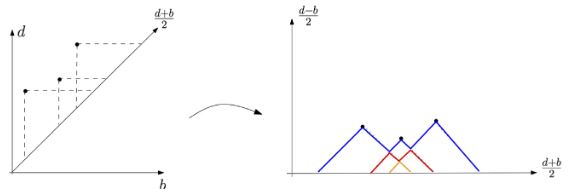
\includegraphics[width=0.85\linewidth]{./figures/Figura12.JPG}
    \caption{
        Ejemplo de un paisaje de persitencia (derecha) asociado con un
        diagrama de persistencia (izquierda).
    }
    \label{fig:Figura 12}
    \vspace{15pt}
\end{figure}

La ventajas de la representaci\'on por paisajes de persistencia son.
Primero, los diagramas de persistencia se convierten en elementos de un espacio funcional,
permitiendo el uso de una variedad m\'as amplia de herramientas de la estad\'istica y
el an\'alisis de datos para el procesamiento de character\'isticas topol\'ogicas,
vease Bubenik (2015)\cite{Bubenik2015}, Chazal et al. (2015)\cite{Chazal2014b}.
Segundo, y fundamental para la perspectiva te\'orica,
los paisajes de persistencia comparten las mismas propiedades de estabilidad
que los diagramas de persistencia (Ver Secci\'on \ref{sec: 4.7}).

\section{Representaciones Lineales de la Persistencia Homol\'ogica}

Un diagrama de persistencia sin su parte escencial puede representarse como
una medida discreta $\delta^{+}=\cllav{p=\cpar{b,d},b<d<\infty}$.
Con un ligero abuso de la notaci\'on, podemos escribir lo siguiente:

\begin{equation*}
    \mathrm{dgm}=\sum_{p\in\mathrm{dgm}}\delta_{p},
\end{equation*}

\noindent donde las caracter\'isticas son contadas con multiplicidad y
$\delta_{\cpar{b,d}}$ denota la medida de Dirac en $p=\cpar{b,d}$.
La mayoria de los descriptores propuestos para analizar la persistencia pueden
ser expresados como transformaciones lineales de un diagrama de persistencia,
vistos como:

\begin{equation*}
    \Psi\cpar{\mathrm{dgm}}=\sum_{p\in\mathrm{dgm}}f\cpar{p},
\end{equation*}

\noindent para alguna funci\'on $f$ definida en $\Delta$ que toma valores en
un espacio de Banach.

En la mayoria de los casos, queremos que estas transformaciones se apliquen de manera
independiente a cada dimensi\'on homol\'ogica. Para $k\in\mathbb{N}$ alguna dimensi\'on
homol\'ogica dada, consideramos alguna transformaci\'on lineal del diagrama de persistencia
restringida a las caracter\'isticas topol\'ogicas de la dimensi\'on $k$ como sigue:

\begin{equation}\label{eq: 4.5}
    \Psi_{k}\cpar{\mathrm{dgm}_{k}}=\sum_{p\in\mathrm{dgm}_{k}}f_{k}\cpar{p},
\end{equation}

\noindent donde $\mathrm{dgm}_{k}$ es el diagrama de persistencia de las caracter\'isticas
topol\'ogicas de la dimensi\'on $k$ donde $f_{k}$ est\'a definido en $\Delta$ y toma valores
en un espacio de Banach.

\section*{Curvas de Betti}

La manera m\'as sencilla de representar la persistencia homol\'ogica es la funci\'n
de Betti o curva de Betti. La curva de Betti de una dimensi\'on homol\'ogica $k$ esta
definida como:

\begin{equation*}
    \beta_{k}\cpar{t}=\sum_{\cpar{b,d}\in\mathrm{dgm}}w\cpar{b,d}\mathds{1}_{t\in\ccorch{b,d}}
\end{equation*}

\noindent donde $w$ es una funci\'on peso definida en $\Delta$. En otras palabras,
la curva de Betti es el n\'umero de cadigos de barra en el tiempo $m$.
Este descriptor es una reapresentaci\'on linear de la homolog\'ia persistente,
tomando $f$ como en (\ref{eq: 4.5}) de forma que
$f\cpar{b,d}\cpar{t}=w\cpar{b,d}\mathds{1}_{t\in\ccorch{bd}}$.
Una elecci\'on t\'ipica para la funci\'on peso es una funci\'on creciente de la persistencia
$w\cpar{b,d}=\tilde{w}\cpar{d-b}$ donde $\tilde{w}$ es una funci\'on creciente definida en $\mathbb{R}^{+}$.
Una de las primeras aplicaciones de las curvas de Betti se puede encontrar en Umeda (2017)\cite{Umeda2017}.

\section*{Superficies de Persistencia}

Una superficie de persistencia (tambi\'en llamadas im\'agenes de persistencia)
se obtiene mediante la convoluci\'on de un diagrama de persistencia con un kernel.
Introducidas en Adams et al. (2017)\cite{Adams2017}. Sea $K:\mathbb{R}^{2}\rightarrow\mathbb{R}$,
un kernel, y $H$ una matriz $2\times 2$ sim\'etrica y definida positiva,
y dada $u\in\mathbb{R}^{2}$ definimos

\begin{equation*}
    K_{H}\cpar{u}=\det\cpar{H}^{-\frac{1}{2}}K\cpar{H^{-\frac{1}{2}}u}.
\end{equation*}

Sea $w:\mathbb{R}^{2}\rightarrow\mathbb{R}_{+}$ una funci\'on peso definida en $\Delta$.
Se define la superficie de persistencia homol\'ogica de dimensi\'on $k$ asociada con el diagrama $\mathrm{dgm}$,
con kernel $K$ y matriz $H$ como sigue:

\begin{equation*}
    \forall u\in\mathbb{R}^{2},
    \rho_{k}\cpar{\mathrm{dgm}}\cpar{u}=
    \sum_{p\in\mathrm{dgm}_{k}}w\cpar{r}K_{H}\cpar{u-p}
\end{equation*}

La superficie de persistencia es entonces una represetaci\'on lineal de la persistencia homol\'ogica.
T\'ipicamente las funciones peso son funciones crecientes de la persistencia.

\section{M\'etricas en el Espacio de Diagramas de Persistencia}
Para aprovechar la informaci\'on y caracter\'isticas topol\'ogicas inferidas por la
homologi\'ia persistente, necesitamos alguna manera de comparar diagramas de persistencia,
esto es, otorgar al espacio de los diagramas de persistencia una estructura de espacio m\'etrico.
Aunque se han considerado una variedad de m\'etricas, la m\'as fundamental de ellas se le conoce como
la distancia de cuello de botella.

\begin{figure}[ht]
    \centering
    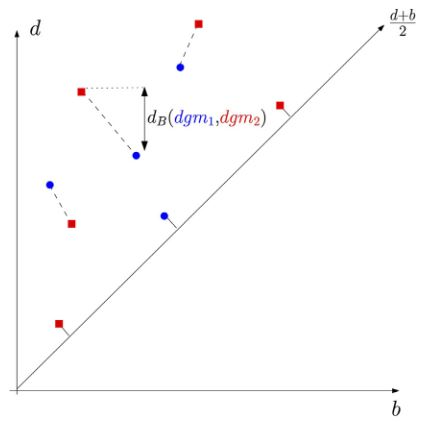
\includegraphics[width=0.85\linewidth]{./figures/Figura13.JPG}
    \caption{
        Emparejamiento perfecto y la distancia de cuello de botella entre un
        diagrama en rojo y un diagrama en azul. N\'otese que algunos puntos
        en ambos diagramas son emparejados a puntos en la diagonal.
    }
    \label{fig:Figura 13}
    \vspace{15pt}
\end{figure}

Recordemos que un diagrama de persistencia es la uni\'on de un multiconjunto discreto
en la parte del plano por encima de la diagonal $\Delta$ y,
por razones t\'ecnicas que veremos adelante,
$\Delta$, donde el punto de $\Delta$ se cuenta con multiplicidad infinita.
Un emparejamiento (ver Figura \ref{fig:Figura 13}) entre dos diagramas,
$\mathrm{dgm}_{1}$ y $\mathrm{dgm}_{2}$, es un subconjunto
$m\subseteq\mathrm{dgm}_{1}\times\mathrm{dgm}_{2}$ tal que cada punto en
$\mathrm{dgm}_{1} - \Delta$ y $\mathrm{dgm}_{2} - \Delta$ aparece exactamente
una vez en $m$.
En otras palabras, para cada $p\in\mathrm{dgm}_{1} - \Delta$ y para cualquier
$q\in\mathrm{dgm}_{2} - \Delta$, $\cpar{\cllav{p}\times\mathrm{dgm}_{2}}\cap m$
y $\cpar{\mathrm{dgm}_{1}\times\cllav{q}}\cap m$ contiene cada uno un \'unico par.
La distancia de cuello de botella entre $\mathrm{dgm}_{1}$ y $\mathrm{dgm}_{2}$
esta definida como

\begin{equation*}
    \mathrm{d}_{\mathrm{b}}\cpar{\mathrm{dgm}_{1},\mathrm{dgm}_{2}} =
    \inf_{\text{empar. }m}\max_{\cpar{p,q}\in m}\cnorm{p-q}_{\infty}.
\end{equation*}

El c\'alculo pr\'actico de la distancia de cuella de botella se resume en
encontrar un cierto emparejamiento perfecto en gr\'aficas bipartitas, y para esto
podemos utilizar algoritmos cl\'asicos.

La distancia de cuello de botella es una m\'etrica parecida a una m\'etrica $\mathit{L}_{\infty}$.
Resulta ser una m\'etrica natural para expresar las propiedades de estabilidad de los
diagramas de persistencia presentados en la secci\'on \ref{sec: 4.7},
pero sufre de las mismas desventajas que las m\'etricas usuales en $\mathit{L}_{\infty}$,
esta completamente determinada por la mayor distancia entre los pares
y no toma en cuenta la cercania de los pares de puntos restantes.
Una variante para superar este problema, es la distancia de Wasserstein entre diagramas.
Dada $p\geq 1$, se define como

\begin{equation*}
    \mathrm{W}_{p}\cpar{\mathrm{dgm}_{1},\mathrm{dgm}_{2}}^{p} =
    \inf_{\text{empar. }m}\sum_{\cpar{p,q}\in m}\cnorm{p-q}_{\infty}^{p}
\end{equation*}

Se han presentado resultados de utilidad acerca de la persistencia en la m\'etrica $\mathrm{W}_{p}$,
particularmente en el estudio por Cohen-Steiner et al. (2010)\cite{Cohen2010},
pero dependen de supuestos que los vuelve consecuencias de los resultados de estabilidad
en la distancia de cuello de botella.
Un estudia general del espacio de diagramas de persistencia dotado con m\'etricas
$\mathrm{W}_{p}$ se ha considerada en Divol y Lacombe (2020)\cite{Divol2021},
donde so propone un marco general basado en transportes parciales \'optimos,
donde muchas propiedades importantes de los diagramas de persistencia pueden probarse de manera natural.

\section{Propiedades de Estabilidad en los Diagramas de Persistencia}\label{sec: 4.7}

Una propiedad fundamental de la homolog\'ia persistente es que
los diagramas de persistencia de filtraciones construidas sobre conjuntos de datos
resultan ser muy estables con respecto a ciertas perturbaciones de los datos.
Para formalizar y cuantificar dichas propiedades, primero necesitamos ser precisos
con respecto a que perturbaciones son permitidas.

En lugar de trabajar directamente con filtraciones sobre conjuntos de datos,
resulta ser m\'as conveniente definir una noci\'on de proximidad entre m\'odulos
de persistencia, de donde derivaremos un resultado de estabilidad general para la
homolog\'ia persistente. Entonces, la mayoria de los resultados de estabilidad
para filtraciones especificas ser\'an consecuencia de este teorema general.
Para evitar discuciones t\'ecnicas y sin p\'erdida de generalidad, suponemos
que los m\'odulos de persistencia considerados est\'an indexados por $\mathbb{R}$.

\begin{definicion}
    Sean $\mathbb{B}$, $\mathbb{W}$ dos m\'odulos de persistencia indexados por
    $\mathbb{R}$. Dado $\delta\in\mathbb{R}$, un homomorfismo de grado $\delta$ entre
    $\mathbb{V}$ y $\mathbb{W}$ es una colecci\'on $\Phi$ de funciones lineales
    $\phi_{r}:V_{r}\rightarrow W_{r+\delta}$, para todo $r\in\mathbb{R}$ tal que
    para cualquier $r\leq s$, $\phi_{r}\circ v_{s}^{r}=w_{s+\delta}^{r+\delta}\circ\phi_{r}$.
\end{definicion}

Un ejemplo importante de un homomorfismo de grado $\delta$ es el endomorfismo de cambio
$\mathrm{1}_{\mathbb{V}}^{\delta}$ el cual consiste de las familias de funciones lineales
$\cpar{v_{r+\delta}^{r}}$. N\'otese que los homomorfismos de m\'odulos pueden ser
naturalmente compuestos; la compisici\'on de un homomorfismo $\Psi$ de grado $\delta$
entre $\mathbb{U}$ y $\mathbb{V}$ y un homomorfismo $\Phi$ de grado $\delta'$ entre
$\mathbb{V}$ y $\mathbb{W}$ naturalmente da lugar a un homomorfismo $\Phi\Psi$ de
grado $\delta + \delta'$ entre $\mathbb{U}$ y $\mathbb{W}$.

\begin{definicion}
    Sea $\delta\geq 0$. Dos m\'odulos de persistencia $\mathbb{V}$, $\mathbb{W}$
    son $delta$-intercalados si existen dos homomorfismos de grado $\delta$,
    $\Phi$, de $\mathbb{V}$ a $\mathbb{W}$ y $\Psi$ de $\mathbb{W}$ a $\mathbb{V}$
    tales que $\Psi\Phi = \mathrm{1}_{\mathbb{V}}^{2\delta}$ y
    $\Phi\Psi = \mathrm{1}_{\mathbb{W}}^{2\delta}$.
\end{definicion}

Aunque no define un am\'etrica en el espacio de los m\'odulos de persistencia,
la noci\'on de cercania entre dos m\'odulos de persistencia puede ser definida como
el m\'as peque\~{n}o $\delta$ no negativo tal que los m\'odulos sean $\delta$-intercalados.
M\'as a\'un, nos ayuda a formalizar el siguiente teorema fundamental
(Chazal et al., 2009\cite{Chazal2009a}; Chazal et al., 2016\cite{Chazal2016a}).

\begin{teorema}[Estabilidad de la persistencia]\label{teo:EstPersist}
    Sean $\mathbb{V}$ y $\mathbb{W}$ dos m\'odulos de persistencia $q$-d\'ociles.
    Si $\mathbb{V}$ y $\mathbb{W}$ son $\delta$-intercalados para alg\'un $\delta>0$,
    entonces
    \begin{equation*}
        \mathrm{d}_{\mathrm{b}}
        \cpar{\mathrm{dgm}\cpar{\mathbb{V}},\mathrm{dgm}\cpar{\mathbb{W}}}\leq\delta.
    \end{equation*}
\end{teorema}

Con este resultado obtenemos una herramienta eficiente para establecer resultados de
estabilidad concretos en el ATD. Por ejemplo, podemos recuperar el primer resultado de
estabilidad de la persistencia que aparece en la literatura
(Cohen-Steiner et al., 2005)\cite{Cohen2005}.

\begin{teorema}
    Sean $f,g:M\rightarrow\mathbb{R}$ dos funciones de valores reales definidas en un
    espacio topol\'ogico $M$ que son $q$-d\'ociles, esto es, que sus filtraciones de
    los conjuntos subnivel de $f$ y $g$ inducen m\'odulos $q$-d\'ociles en el nivel de
    la homolog\'ia. Entonces, para cualquier entero $k$,
    \begin{equation*}
        \mathrm{d}_{\mathrm{b}}
        \cpar{\mathrm{dgm}_{k}\cpar{f},\mathrm{dgm}_{k}\cpar{g}}\leq
        \cnorm{f-g}_{\infty}=
        \sup_{x\in M}\cabs{f\cpar{x}-f\cpar{x}}
    \end{equation*}
    donde $\mathrm{dgm}_{k}\cpar{f}$ es el diagrama de persistencia de el m\'odulo
    de persistencia $\cpar{H_{k}}\cpar{f^{-1}\cpar{-\infty,r}}|r\in\mathbb{R}$,
    y respectivamente para $\mathrm{dgm}_{k}\cpar{f}$,
    donde las funciones lineales son las inducidas por las inclusiones can\'onicas
    entre los conjuntos subnivel.
\end{teorema}
\begin{prueba}
    Denotamos $\delta=\cnorm{f-g_{\infty}}$, tenemos que para cualquier $r\in\mathbb{R}$,
    $f^{-1}\cpar{-\infty,r}\subseteq g^{-1}\cpar{-\infty,r+\delta}$ y
    $g^{-1}\cpar{-\infty,r}\subseteq f^{-1}\cpar{-\infty,r+\delta}$.
    este intercalado entre los conjuntos subnivel de f induce un $\delta$-intercalamiento
    entre los m\'odulos de persistencia en el nivel de la homolog\'ia,
    y as\'i, el resultado se sigue de una aplicaci\'on directa del teorema anterior.
\end{prueba}

El \emph{Teorema \ref{teo:EstPersist}} tambi\'en implica el siguiente resultado
de estabilidad para los diagramas de persistencia de filtraciones construidas sobre
conjuntos de datos.

\begin{teorema}\label{teo:4.9}
    Sean $\mathbb{X}$ y $\mathbb{Y}$ dos espacios m\'etricos compactos y sean
    $\mathrm{Filt}\cpar{\mathbb{X}}$ y $\mathrm{Filt}\cpar{\mathbb{Y}}$ las
    filtraciones de Vietoris-Rips o de \v Cech contruidos sobre $\mathbb{X}$ y
    $\mathbb{Y}$. Entonces
    \begin{equation*}
        \mathrm{d}_{\mathrm{b}}
        \cpar{\mathrm{dgm}\cpar{\mathrm{Filt}\cpar{\mathbb{X}}},
        \mathrm{dgm}\cpar{\mathrm{Filt}\cpar{\mathbb{Y}}}}\leq
        2\mathrm{d}_{\mathrm{GH}}\cpar{\mathbb{X},\mathbb{Y}}
    \end{equation*}
    donde $\mathrm{dgm}\cpar{\mathrm{Filt}\cpar{\mathbb{X}}}$ y
    $\mathrm{dgm}\cpar{\mathrm{Filt}\cpar{\mathbb{Y}}}$ denotan los
    diagramas de persistencia de las filtraciones $\mathrm{Filt}\cpar{\mathbb{X}}$ y
    $\mathrm{Filt}\cpar{\mathbb{Y}}$.
\end{teorema}

Como notamos en el Ejemplo 3 de la Secci\'on \ref{sec: 4.2}, los diagramas de persistencia pueden
ser interpretados como character\'isticos topol\'ogicos multiescala de 
$\mathbb{X}$ y $\mathbb{Y}$. Adem\'as, el Teorema \ref{teo:4.9} nos dice que estos
character\'isticos son resilientes con respecto a perturbaciones de los datos en la
m\'etrica de Gromov-Hasudorff. As\'i, pueden ser usados como propiedades discriminatorias
para tareas de clasificaci\'on entre otras (vease, por ejemplo, Chazal et al. (2009)\cite{chazal2009b}
para un aplicaci\'on a la clasificaci\'on no r\'igida de figuras 3D).

Ahora damos resultados similares para la representaciones alternativas de la homolog\'ia
persistente que vimos con anterioridad. De la definici\'on de paisajes de persistencia,
obsevamos que $\lambda\cpar{k,\cdot}$ es $1$-Lipschitz, y esto es suficiente para que
propiedades de estabilidad similares a las de los diagramas de persistencia se satisfagan
para los paisajes.

\begin{proposicion}[Estabilidad de los paisajes de persistencia; Bubenik (2015)\cite{Bubenik2015}]
    Sean $\mathrm{dgm}$ y $\mathrm{dgm}'$ dos diagramas de persistencia (sin sus partes escenciales).
    Para cualquier $t\in\mathbb{R}$ y cualquier $k\in\mathbb{N}$, tenemos lo siguiente:

    \begin{enumerate}[label=(\roman*)]
        \item $\lambda\cpar{k,t}\geq\lambda\cpar{k+1,t}\geq 0$.
        \item $\cabs{\lambda\cpar{k,t}-\lambda'\cpar{k,t}}\geq
        \mathrm{d}_{\mathrm{b}}\cpar{\mathrm{dgm},\mathrm{dgm}'}$.
    \end{enumerate}
\end{proposicion}

Una amplia gama de representaciones lineales es continua con respecto a la m\'etrica
de Wasserstein $\mathrm{W}_{s}$ en el espacio de los diagramas de persistencia y
con respecto a la norma de Banach para las representaciones lineales de la persistencia.
En general, no suempre es posible dar una cota superior para el m\'odulo de continuidad
del operador de representaciones lineales. Sin embargo, en el caso donde $s=1$, es posible
probar adem\'as un resultado de estabilidad si la funci\'on de peso toma valores peque\~{n}os
para puntos cercanos a la diagonal. (vease Divol y Lacombe (2020)\cite{Divol2021},
Hofer et al. (2019)\cite{Hofer2019b}).

\section*{La Estabilidad y la Capacidad Discriminativa de las Representaciones de Persistencia}

Los resultados en el estudio por Divol y Lacombe (2020)\cite{Divol2021} muestran que
la continuidad y estabilidad solo son posible con funciones de pesos que toman valores peque\~{n}os
para puntos cercanos a la diagonal. No obstante, en general, no hay raz\'on espec\'ifica para
considerar que los puntos cercanos a la diagonal son menos importantes, dada alguna tarea de aprendizaje.
Desde una perspectiva del aprendizaje autom\'atico, tambi\'en es relevante dise\~{n}ar
representaciones lineales con funciones de peso generales, aunque seria m\'as dif\'icil probar
la consistencia de los m\'etodos correspondientes sin al menos la continuidad de la representaci\'on.
Si bien la estabilidad estabilidad es importante, es quiz\'as un requisito muy fuerte
para muchos de los problemas en la ciencia de datos.
Posiblemente, dise\~{n}ar representaciones lineales que sean sensibles a partes espec\'ificas de los
diagramas de persistencia, sea una mejor estrategia en la pr\'actica
que buscar la estabilidad global de la representaci\'on.

\chapter{Aspectos Estad\'isticos de la Homolog\'ia Persistente}\label{chap:Cap5}cap 5

Por s\'i sola, la homolog\'ia persistente no toma en cuenta la naturaleza estoc\'astica de los datos
y la variabilidad intrinseca de las cantidades topol\'ogicas que infieren.
Buscamos ahora un acercamiento esta\'distico a la homolog\'ia persistente,
considerando que los datos son generados de alguna distribuci\'on desconocida.
Comenzamos dando varos resultados de consistencia para la inferencia de la homolog\'ia persistente.

\section{Resultados de Consistencia para la Homolog\'ia Persistente}

Sup\'ongase que observamos $n$ puntos $\cpar{X_{1},\dots,X_{n}}$ en un espacio m\'etrico
$\cpar{M,\rho}$ obtenidas i. i. d. de una medida de probabilidad desconocida $\mu$ con
soporte compacto $\mathbb{X}_{\mu}$ la distancia de Gromov-Hausdorff nos permite comparar
$\mathbb{X}_{\mu}$ con otros espacios m\'etricos compactos no necesariamente encajados en $M$.
Definimos a continuaci\'on, $\hat{\mathbb{X}}$ un estimador de $\mathbb{X}_{\mu}$
como una funci\'on de $X_{1},\dots,X_{n}$ que toma valores en el conjunto de espacios
m\'etricos compactos.

Sean $\mathrm{Filt}\cpar{\mathbb{X}_{\mu}}$ y $\mathrm{Filt}\cpar{\hat{\mathbb{X}}}$
dos filtraciones definidas en $\mathbb{X}_{\mu}$ y $\hat{\mathbb{X}}$.
Con el teorema \ref{teo:4.9} hemos visto que una estrategia natural
para estimar la homologi\'ia persistente de $\mathrm{Filt}\cpar{\mathbb{X}_{\mu}}$
consiste en estimar el soporte de $\hat{\mathbb{X}}$.
N\'otese que en algunos casos, el espacio $M$ puede ser desconocido
y las observaciones $X_{1},\dots,X_{n}$ solo se conocen mediante de sus distancias por pares
$\rho\cpar{X_{i}, X_{j}}$, $i$, $j = 1,\dots,n$.
La distancia de Gromov-Hausforff nos permite considerar el conjunto de observaciones
como un espacio m\'etrico abstracto de cardinalidad $n$,
independietemente de la manera en la que esta encajado en $M$.
Esta estructura general incluye el acercamiento m\'as est\'andar
que consiste en estamar el soporte con respecto a la distancia de Hausdorff
restringiendo los valores de $\hat{\mathbb{X}}$ a los conjuntos compactos en $M$.

El conjunto finito $\mathbb{X}_{n}:=\cllav{X_{1},\dots,X_{2}}$
es un estimador natural para el soporte de $\mathbb{X}_{\mu}$.
En muchos de los contextos que veremos a continuaci\'on,
$\mathbb{X}_{\mu}$ muestra tasas de convergencia \'optimas
con respecto a la ditancia de Hausdorff.
Para algunas constantes $a,b>0$, decimos que $\mu$ satisface el supuesto
$\cpar{a,b}$-est\'andar si para cualquier $x\in\mathbb{X}_{\mu}$ y cualquer $r>0$,
\begin{equation}
    \mu\cpar{B\cpar{x,r}}\geq\min\cpar{ar^{b},1}.
\end{equation}

Este supuesto es ampliamente usado en la literatura de la estimaci\'on de conjuntos
bajo la distancia de Hausdorff
(Cuevas y Rodriguez-Casal, 2004\cite{CuevasRodriguezCasal2004};
Singh et al., 2009\cite{Singh2009}).
Bajo este supuesto, puede deducirse que la tasa de convergencia de
$\mathrm{dgm}\cpar{\mathrm{Filt}\cpar{\mathbb{X}_{n}}}$ a
$\mathrm{dgm}\cpar{\mathrm{Filt}\cpar{\mathbb{X}_{\mu}}}$
para la m\'etrica de cuello de botella es acotada superiormente por
$O\cpar{\frac{\log n}{n}}^{1/b}$. M\'as precisamente, esta tasa
acota superiormente la tasa de convergencia minimax sobre el conjunta de medidas
de probabilidad en el espacio m\'etrico $\cpar{M, \rho}$ satisfaciendo el supuesto
$\cpar{a,b}$-est\'andar en $M$.

\begin{teorema}
    Chazal et al. (2014)\cite{Chazal2014b} para algunas constantes positivas, $a$ y $b$, sea
    \begin{equation*}
        \mathcal{P}:=\cllav{\mu \text{ en } M |
        \mathbb{X}_{\mu}\text{ es compacto y }\forall x\in\mathbb{X}_{\mu},\forall r>0,\hspace{4pt}
        \mu\cpar{B\cpar{x,r}}\geq\min\cpar{1,ar^{b}}}
    \end{equation*}
    Entonces, se tiene que
    \begin{equation*}
        \sup_{\mu\in\mathcal{P}}\mathbb{E}\ccorch{
        \mathrm{d}_{\mathrm{b}}\cpar{\mathrm{dgm}\cpar{\mathrm{Filt}\cpar{\mathbb{X}_{\mu}}},
        \mathrm{dgm}\cpar{\mathrm{Filt}\cpar{\mathbb{X}_{n}}}}}\leq
        C\cpar{\frac{\log n}{n}}^{1/b}
    \end{equation*}
    Donde la constante $C$ depende solo de $a$ y $b$.
\end{teorema}

Bajo algunos supuestos t\'ecnicos adicionales, se pueden evidenciar las cotas inferiores correspondientes
(hasta un t\'ermino logar\'itmico) (vease Chazal et al. (2014)\cite{Chazal2014b}).
Utilizando resultados de estabilidad, se pueden obtener resultados de consistencia similares
bajo modelos generativos alternativos siempre que se conosca un estimador del soporte
consistente bajo la m\'etrica de Hausdorff.
Por ejemplo, de los resultados del estudio por Genovese et al. (2012)\cite{Genovese2012}
sobre la estimaci\'on del soporte Hausforff bajo ruido aditivo,
se puede deducir que las tasas de convergencia minimax para la estimaci\'on de diagramas de persistecia
son m\'as r\'apidas que $\cpar{\log n}^{-1/2}$.
M\'as a\'un, siempre que se disponga de un resultado de estabilidad para alguna representaci\'on de la persistencia dada,
resultados de consistencia similares pueden ser directamente derivados de la consistencia de diagramas de persistencia.

\section*{Estimaci\'on de la Homolog\'ia Persistente de Funciones}

El Teorema \ref{teo:EstPersist} abre la puerta a la estimaci\'on
de la homolog\'ia persistente en funciones definidas en $\mathbb{R}^{d}$,
en una subvariedad de $\mathbb{R}^{d}$ o, m\'as generalmente, en un espacio m\'etrico.
La homolog\'ia persistente de funciones de regresi\'on a sido estudiada por
Bubenik et al. (2010)\cite{Bubenik2010}.
El acercamiento alternativo de Bobrowski et al. (2014)\cite{Bobrowski2014},
basado en la inclusi\'on entre pares anidados de los conjuntos de nivel estimados,
puede aplicarse con estimadores del kernel de regresi\'on y de la densidad del kernel
para estimar la homolog\'ia persistente de funciones de densidad y regresi\'on.
Otra rama de investigaci\'on en este tema trata con varias versiones robustas de ATD.
Una soluci\'on es estudiar la homolog\'ia persistente de de los conjuntos super-nivel
de estimadores de densidad (Fasy et al., 2014\cite{Fasy2014b}).
Otra alternativa, m\'as estrechamente relacionada a la funci\'on distancia, pero robusta al ruido,
consiste en estudiar la homolog\'ia persistente de conjuntos subnivel de la distancia

a una medida definida en la secci\'on \ref{sec: 3.3} (Chazal et al., 2017\cite{Chazal2017}).
\section{Estad\'isticos de la Homolog\'ia Persistente Calculados en una Nube de Puntos}

Para muchas aplicaciones,
en especial donde el soporte de la nube de puntos no esta dibujado sobre o es cercano a una figura geom\'etrica,
los diagramas de persistencia pueden ser dif\'iciles de analizar.
En particular, muchos caracter\'isticos topol\'ogicos estan cerca de la diagonal.
Como corresponden  a estructuras topol\'ogicas que viven por un periodo muy corto de tiempo,
estos puntos son generalmente considerados ruido (ver Figura \ref{fig:Figura 14}).
Las regiones de confianza para los diagramas de persistencia nos otorgan una respuesta
de rigor al problema de distingir entre la se\~{n}al y el ruido en estas representaciones.

Los resultados de estabilidad dados en la secci\'on \ref{sec: 4.7}
motivan el uso de la distancia de cuello de botella para definir regiones de confianza.
Sin embargo, distancias alternativas inspiradas en distancias de Wasserstein tambi\'en pueden ser propuestas.
Cuando se estima un diagrama de persistecia $\mathrm{dgm}$ con un estimador $\widehat{\mathrm{dgm}}$,
buscamos un valor $\eta_{\alpha}$ tal que

\begin{equation*}
    P\cpar{\mathrm{d}_{\mathrm{b}}\cpar{\widehat{\mathrm{dgm}},\mathrm{dgm}}\geq\eta_{\alpha}}\leq\alpha,
\end{equation*}

para $\alpha\in\cpar{0,1}$. Sea $\mathrm{B}_{\alpha}$ la bola cerrada de radio $\alpha$
para la distancia de cuello de botella, centrada en $\widehat{\mathrm{dgm}}$ en el espacio
de los diagramas de persistencia. Siguiendo a Fasy et al. (2014)\cite{Fasy2014b},
podemos visualizar los puntos que pertenecen a esta bola de varias maneras.
Una primera opci\'on es centrar una caja con lados de largo $2\alpha$
en cada punto del diagrama $\widehat{\mathrm{dgm}}$.
Una soluci\'on alternativa es visualizar el conjunto de confianza
a\~{n}adiendo una banda a una distancia $\eta_{\alpha}/2$ de la diagonal
(siendo la distancia de cuello de botella definida para la norma $\ell_{\infty}$)
(ver Figura \ref{fig:Figura 14} para una ilustraci\'on).
Luego los puntos fuera de la banda son considerados, cualidades topol\'ogicas significativas
(v\'ease el estudio por Fasy et al. (2014)\cite{Fasy2014b} para m\'as detalles).

\begin{figure}[ht]
    \centering
    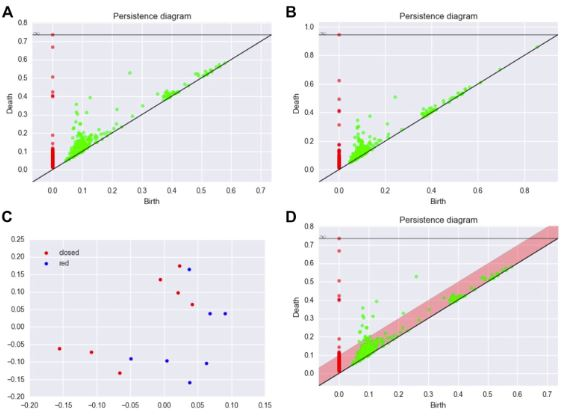
\includegraphics[width=0.85\linewidth]{./figures/Figura14.JPG}
    \caption{
        (A, B) Dos diagramas de persistencia para dos configuraciones de la MBP
        (Maltose-Binding Protein).
        (C) Configuraci\'on MDS (Multi-Dimensional Scaling)
        para la matriz de distancias de cuello de botella.
        (D) Diagrama de persistencia con regi\'on de confianza para la MBP.
    }
    \label{fig:Figura 14}
    \vspace{15pt}
\end{figure}

Se han propuesto una variedad de m\'etodos para estimar $\eta_{\alpha}$
en el estudio por Fasy et al. (2014)\cite{Fasy2014b}.
Estos m\'etodos recaen principalmente en los resultados de estabilidad
para diagramas de persistencia;
se pueden derivar conjuntos de confianza para diagramas
de los conjuntos de confianza en el espacio muestral.

\subsection*{Acercamiento por submuestreo}

Este m\'etodo se basa en una regi\'on de confianza para el soporte $K$
de la distribuci\'on de la muestra en la distancia de Hausdorff.
Sea $\tilde{\mathbb{X}_{b}}$ un submuestreo de tama\~{n}o $b$ de una muestra
$\tilde{\mathbb{X}_{n}}$, donde $b = o\cpar{n/\log n}$.
Sea $\mathrm{q}_{b}\cpar{1 - \alpha}$ un cuantil de la distribuci\'on de
$\mathrm{Haus}\cpar{\tilde{\mathbb{X}_{b}},\mathbb{X}_{n}}$.
Sea $\Hat{\eta}_{\alpha}:=2\Hat{q}_{b}\cpar{1-\alpha}$, donde
$\Hat{q}_{b}$ es una estimaci\'on $\mathrm{q}_{b}\cpar{1-\alpha}$ usando un
procedimiento de Monte Carlo est\'andar.
Bajo un supuesto $\cpar{a,b}$ est\'andar y para una $n$ suficientemente grande,
el estudio por Fasy et al. (2014)\cite{Fasy2014b} muestra que

\begin{equation*}
    P\cpar{
        \mathrm{d}_{b}\cpar{
            \mathrm{dgm}\cpar{\mathrm{Filt}\cpar{K}},
            \mathrm{dgm}\cpar{\mathrm{Filt}\cpar{\mathbb{X}_{n}}}
        }
        >\Hat{\eta}_{\alpha}
    }
    \leq
    P\cpar{
        \mathrm{Haus}\cpar{K,\mathbb{X}_{n}}>\Hat{\eta}_{\alpha}
    }
    \leq
\alpha+O\cpar{\frac{b}{n}}^\frac{1}{4}.
\end{equation*}

\section*{Bootstrap de Cuello de Botella}

Los resultados de estabilidad suelen llevar a conjuntos de confianza conservativos.
Una estrategia alternativa es el bootstrap de ceullo de botella
introducido en el estudio por Chazal et al. (2016)\cite{Chazal2016a}.
Consideramos el escenario general donde un diagrama de persistencia
$\Hat{\mathrm{dgm}}$ se define como la observaci\'on
$\cpar{X_{1},\dots,X_{n}}$ en un espacio m\'etrico.
Este diagrama de persistencia corresponde a la estimaci\'on de
un diagrama de persistencia subyacente $\mathrm{dgm}$,
que puede ser relacionado, por ejemplo, al soporte de la medida,
o al los conjutos subnivel de la funci\'on relacionada a esta distribuci\'on
(Por ejemplo, una funci\'on de densidad donde las $X_{i}$'s estan en
$\mathbb{R}^{d}$).
Sea $\cpar{X_{1}^{*},\dots,X_{n}^{*}}$ una muestra de una medida emp\'irica
definida de las observaciones $\cpar{X_{1},\dots,X_{n}}$.
Y sea $\widehat{\mathrm{dgm}}^{*}$ el diagrama de persistencia
derivado de esta muestra.
Podemos tomar entonces para $\eta_{\alpha}$ la cantidad $\Hat{\eta}_{\alpha}$
definida por:
\begin{equation}
    P\cpar{\mathrm{d_{b}}\cpar{
    \widehat{\mathrm{dgm}}^{*},\widehat{\mathrm{dgm}}}>\widehat{\eta}_{\alpha}|X_{1},\dots,X_{n}} 
    =\alpha.
\end{equation}
Es de notar que $\Hat{\eta}_{\alpha}$ puede ser estimada con facilidad utilizando
m\'etodos de Monte Carlo.
Se ha demostrado en el estudio por Chazal et al. (2016)\cite{Chazal2016b}
que el bootstrap de cuello de botella es una opci\'on v\'alida para calcular
los conjuntos subnivel de un estimador de densidad.

\section*{Bootstrap para N\'umeros de Betti Persistentes}

Como se ha mencionado, las regiones de confianza basadas en las propiedades de estabilidad
de la persistencia suelen dar lugar a regiones de confianza muy conservadoras.
Basados en los conceptos de estad\'isticos estabilizantes, Penrose y Yukick
(2001)\cite{PenroseYukich2001}, recientemente si ha mostrado normalidad asint\'otica para
n\'umeros de Betti persistentes en Krebs y Polonik (2019)\cite{KrebsPolonik2019},
y en Roycraft et al. (2020)\cite{Roycraft2020} bajo muy pocas condiciones en la filtraci\'on y
distribuci\'on de la nube muestral.
Adem\'as los procedimientos de bootstrapping tambi\'en son v\'alidos en este
acercamiento.
M\'as precisamente, un procedimiento bootstrap suavizado junto a un conveniente
reescalado de la nube de puntos, parece ser un acercamiento prometedor
para el bootstrapping de caracter\'isticas ATD de la nube de puntos de datos.

\section{Estad\'isticos para una Familia de Diagramas de Persistencia y Otras Representaciones}

Hasta ahora hemos considerado estad\'isticos basados solamente un diagrama de persistencia.
Dirigimos nuestra atenci\'on ahora a un nuevo esquema donde se encuentran a disposici\'on una
variedad de diagramas de persistencia (y otras representaciones),
y estamos interesados en proveer una tendencia central,
regiones de confianza y pruebas de hip\'otesis para descriptores topol\'ogicos
construidos en esta familia.

\subsection{Tendencia Central para la Homolog\'ia Persistente}

\textbf{\textit{\large Media de Distribuciones de Diagramas}}

Dado que el espacio de diagramas de persistencia es un espacio m\'etrico general pero no
un espacio de Hilbert, la definici\'on de media en diagramas de persistencia no es obvia ni
\'unica.
Un primer acercamiento natural para definir una medida de tendencia central en este contexto
es considerar la media de Fr\'echet de distribuciones de diagramas.
Su existencia ha sido demostrada en el estudio por Mileyko et al. (2011)\cite{Mileyko2011},
y tambi\'en han sido caracterizadas en el estudio por Turner er al. (2014)\cite{Turner2014a}.
Sin embargo, pueden no ser \'unicas, y resultan complicadas de calcular en la pr\'actica.
Algunos acercamientos para tratar de solucionar estas problematicas que se han propuesto
recientemente incluyen la propuesta basada en transporte \'optimo n\'umerico
Lacombe et al. (2018)\cite{Lacombe2018} as\'i como las representaciones lineales y m\'etodos
basados en el kernel por Divol y Chazal (2020)\cite{Divol2020}.\medbreak\medbreak

\textbf{\textit{\large Firmas Topol\'ogicas de Submuestras}}

Tambi\'en podemos usar propiedades de tendencia central de la homolog\'ia persistente para
calcular firmas topol\'ogicas para conjuntos de datos de gran tama\~{n}o,
como alternativa al prohibitivo costo de los c\'alculos de persistencia.
Dada una gran nube de puntos, la idea es extraer muchas submuestras,
calcular el paisaje de persistencia de cada submuestra, y luego combinar la informaci\'on.

Para cualquier entero positivo $m$, sea $X = \cllav{X_{1},\dots,x_{m}}$ un muestra de $m$ puntos
tomada de una medida $\mu$ en un espacio m\'etrico $M$
cuyo soporte es denotado por $\mathbb{X}_{\mu}$.
Suponemos que el diametro de $\mathbb{X}_{\mu}$ es finito
y acotado superiormente por $\frac{T}{2}$,
donde $T$ es la misma constante que en la definici\'on de paisajes de persistencia
en la Secci\'on \ref{sec: 4.4}.
Concentramos nuestra atenci\'on ahora en el caso de $k=1$ y el conjunto
$\lambda\cpar{t}=\lambda\cpar{1,t}$.
Sin embargo, los resultados que presentaremos a continuaci\'on se sostienen para $k>1$.
El paisaje de persistencia correspondiente (asociado con el diagrama de persistencia
de la filtraci\'on de \v Cech o Vietoris-Rips) es $\lambda_{X}$
y denotamos por $\psi_{\mu}^{m}$ la medida inducida por $\mu^{\otimes m}$
en el espacio de paisajes de persistencia.
N\'otese que el paisaje de persistencia $\lambda_{X}$ puede ser visto como
una \'unica muestra de la medida $\lambda_{\mu}^{m}$.
La esperanza puntual del paisaje de persistencia (aleatorio) bajo esta medida
se define por $\mathbb{E}_{psi_{\mu}^{m}}\ccorch{\lambda_{X}\cpar{t}}, t\in\ccorch{0,T}$.
El paisaje promedio $\mathbb{E}_{psi_{\mu}^{m}}\ccorch{\lambda_{X}}$
tiene una contraparte emp\'irica natural, que puede ser usada como un estimador insesgado.
Sea $S_{1}^{m},\dots,S_{\ell}^{m}$, $\ell$ muestras independientes de
tama\~{n}o $m$ de $\lambda^{\otimes m}$. Definimos el paisaje emp\'irico promedio como

\begin{equation}
    \overline{\lambda_{\ell}^{m}}\cpar{t}=
    \frac{1}{b}\sum_{i=1}^{b}\lambda_{S_{i}^{m}}\cpar{t},\text{ para todo }t\in\ccorch{0,T},
\end{equation}

y proponemos usar $\overline{\lambda_{\ell}^{m}}$ para estimar $\lambda_{\mathbb{X}_{\mu}}$.
N\'otese que calcular la homolog\'ia persistente de $\mathbb{X}_{n}$ es
$O\cpar{\mathrm{exp}\cpar{n}}$,
mientras que calcular la del paisaje promedio es $O\cpar{b\hspace{3pt}\mathrm{exp}\cpar{n}}$.

Otra motivaci\'on para este acercamiento por submuestreos es que
tamb\'ien puede ser aplicado cuando $\mu$ es una medida discreta con el soporte
$\mathbb{X}_{N}=\cllav{x_{1},\dots,x_{N}}$ en el espacio m\'etrico $M$.
Lo anterior es muy com\'un en la pr\'actica, cuando una medida continua (pero desconocida)
es aproximada par una medida uniforme discreta $\mu_{N}$ en $\mathbb{X}_{N}$.


El paisaje promedio $\mathbb{E}_{\psi{\mu}^{m}}\ccorch{\lambda_{X}}$ es interesante por si mismo,
ya que trae contiene cierta informaci\'on topol\'ogica estable
acerca de la medida subyacente $\mu$,
de la cual se generan los datos.

\begin{teorema}
    [Chazal et al. (2015a)\cite{Chazal2015a}] Sea $X\sim\mu^{\otimes m}$ y
    $Y\sim\nu^{\otimes m}$, donde $\mu$ y $\nu$ son dos medidas de probabilidad en $M$.
    Para cualquier $p\geq 1$, tenemos
    \begin{equation*}
        \cnorm{\mathbb{E}_{\psi_{\mu}^{m}}\ccorch{\lambda_{X}}-
        \mathbb{E}_{\psi_{\nu}^{m}}\ccorch{\lambda_{Y}}}_{\infty}\leq
        2 m^{\frac{1}{p}} \mathrm{W}_{p}\cpar{\mu,\nu},
    \end{equation*}
    donde $\mathrm{W}_{p}$ es la $p$-\'esima distancia de Wasserstein en $M$.
\end{teorema}

Lo anterior nos resulta \'util por dos razones. Primero, nos dice que para una $m$ fija,
el ``comportamiento topol\'ogico'' del conjunto de $m$ puntos
trae consigo cierta informaci\'on estable sobre la medida subyacente de la cual se
generan los datos.

\subsection{Normalidad Asint\'otica}

Como en la secci\'on anterior, consideramos una multitud de diagramas de persistencia
(o alguna otra representaci\'on). El siguiente paso despues de dar descriptores
de tendencia central para la persistencia homol\'ogica es proveer resultados de
normalidad asint\'otica, as\'i como procesos bootstrap para ser capaces de derivar
intervalos de confianza. Por supuesto, resulta m\'as sencillo otorgar resultados para
representaciones funcionales de la persistencia. En los estudios por
Chazal et al. (2015a)\cite{Chazal2015b}, Chazal et al. (2015c)\cite{Chazal2015c},
siguiendo esta estrategia, se proponen bandas de confianza para paisajes a partir de
observaciones de paisajes $\lambda_{1},\dots,\lambda_{N}$ obtenidas i. i. d. de
una distribuci\'on aleatoria en el espacio de paisajes.
La validez asint\'otica y la convergencia uniforme del multiplicador bootstrap
se demuestra en este marco.
N\'otese que resultados similares tambi\'en se han propuesto para muchas otras representaciones
de la persistencia, en particular provando que los espacios funcionales correspondientes son
espacios de Donsker.

\section{Otros Acercamientos Estad\'isticos al An\'alisis Topol\'ogico de Datos}

Se ha mostrado un aumento en el inter\'es por acercamientos estad\'isticos al ATD
y se han propuesto y estudiado varios en los a\~{n}os recientes, a continuaci\'on
una lista no exhaustiva de ejemplos.

\textbf{\large Prueba de Hip\'otesis}

Se han propuesto varios m\'etodos para procedimientos de prueba de hip\'otesis
para la persistencia homol\'ogica, en su mayor\'ia para pruebas de dos muestras y
basados en estrategias de permutaci\'on.
Robinson y Turner (2017)\cite{Robinson2017} se concentran en distancias por pares
de diagramas de persistencia, mientras que Berry et al. \cite{Berry2020}
estudian acercamientos m\'as generales.
Tamb\'ien se han propuesto pruebas de hip\'otesis basadas en
acercamientos enfocados en el kernel en el estudio por Kusano (2019)\cite{Kusano2019}.
Adem\'as una prueba de hip\'otesis de dos etapas de filtraci\'on y prueba para imagenes de
persistencia fue presentada en el estudio por
Moon y Lazar (2020)\cite{Moon2020}.\medbreak\medbreak

\textbf{\large Transformada de la Homolog\'ia Persistente}

Las representaciones introducidas anteriormente son todas transformaciones derivadas
del diagrama de persistencia calculado de una filtraci\'on fija construida sobre
un conjunto de datos.
La transformada de la homlog\'ia persistente introducida en los estudios por
Curry et al. (2018)\cite{Curry2018}, Turner et al. (2014b)\cite{Turner2014b}
para estudiar figuras en $\mathbb{R}^{d}$
toma un camino diferente enfocandose en la homolog\'ia persistente del
conjunto subnivel de la filtraci\'on inducida por la proyecci\'on de la figura
considerada en cada direcci\'on de $\mathbb{R}^{d}$.
Tiene varias propiedades interesantes; en particular, la transformada de la
homolog\'ia persistente es un estad\'istico suficiente para distribuciones definidas en
el conjunto de complejos simpliciales geom\'etricos y finitos,
encajados en $\mathbb{R}^{d}$. \medbreak\medbreak

\textbf{\large Estad\'istica Bayesiana para el An\'alisis Topol\'ogico de Datos}

Se ha propuesto un acercamiento Bayesiano a la inferencia de diagramas de persistencia
en el estudio por Maroulas et al. (2020)\cite{Maroulas2020}
que consiste en entender un diagrama de persistencia como una muestra de un proceso puntual.
Este m\'etodo Bayesiona calcula la intensidad posterior del proceso puntual basado en
una intensidad de mezcla Gaussiana para el previo.

\section{Homolog\'ia Persistente y el Aprendizaje Auto\'matico}

Usando el ATD y, m\'as especificamente, la homolog\'ia persistente para el
apredizaje autom\'atico ha sido un tema de alto muy alto inter\'es que ha
generado amplia e intensa investigaci\'on.
Aunque los avances recientes se escapan el alcance de este trabajo,
introducimos a continuaci\'on las pricipales direcciones que la investigaci\'on
ha tomado con algunas referencias de inter\'es particular. \medskip\medskip

\textbf{\large An\'alisis Topol\'ogico de Datos para
Exploraci\'on de Datos y Estad\'isticos Descriptivos}

In algunos dominios, el ATD puede ser usado como una herramienta para el an\'alisis exporatorio
y la visualizaci\'on.
Por ejemplo, el algoritmo Mapper provee un acercamiento poderoso para explorar y visualizar
la estructura topol\'ogica global de conjuntos de datos intricados.
En algunos casos, diagramas de persistencia obtenidos de datos pueden ser directamente
interpretados y explotados para el mejor entendimiento del fen\'omeno del cual los
datos han sido generados.
Este es el caso en el estudio sobre campos de fuerza en medios granulares
(Kramar et al., 2013\cite{Kramar2013}) o en el de las estructuras at\'omicas en vidrio
(Nakamura et al., 2015\cite{Nakamura2015}) en la ciencia de materiales,
en el estudio de la evoluci\'on de patrones de convecci\'on en la din\'amica de fluidos
(Kram\'ar et al., 2016\cite{Kramar2016}), y en el monitoreo maquinista
(Khasawneh y Munch, 2016\cite{Khasawneh2016}) o en el an\'alisis de estructuras
nanoporosas en qu\'imica (Lee et al., 2017\cite{Lee2017}) donde caracter\'isticas
topol\'ogicas pueden ser relacionadas con estructuras geom\'etricas topol\'ogicas
y patrones en los datos considerados.\medskip\medskit


\textbf{\large Homolog\'ia Persistente para la Ingenieria de Caracter\'isticas}

Hay muchas otros casos de las car\'acteristicas de la persistencia no pueden ser
directamente interpretadas de manera sencilla, sin embargo, existe informaci\'on de valor
en ellas que requiere un procesamiento adicional.
No obstante, la naturaleza altamente no lineal de los diagramas de persistencia
nos impide usarlos de manera inmediata como caracter\'isticas est\'andar en algoritmos de
aprendizaje autom\'atico.

Los paisajes de persistencia y sus representaciones lineales ofrecen una primera opci\'on
para convertir diagramas de persistencia en elementos de un espacio vectorial que pueden ser
directamente usados  como caracter\'isticas en los esquemas cl\'asicos de
aprendizaje autom\'atico.
Ese acercamiento ha sido utilizado, por ejemplo, en la uni\'on de proteinas
(Kovacev-Nikolic et al., 2016\cite{Kovacev2016}), reconocimiento de objetos
(Li et al., 2014\cite{Li2014}), o en el an\'alisis de series de tiempo.
De manera similar, la construcci\'on de kernels para diagramas de persistencia
que preservan las propiedades de estabilidad a sido objeto de atenci\'on recientemente.
La mayoria de ellos han sido obtenidos considerando diagrams como medidas discretas en
$\mathbb{R}^{2}$.
Convolucionando una versi\'on simetrizada (con respecto a la diagonal)
de los diagramas de persistencia con una distrivuci\'on Gaussiana $2$-dimensional,
Reininghaus et al. (2015)\cite{Reini2015} introdujo un kernel multiescala y lo aplic\'o
a la clasificaci\'on de figuras y problemas de reconocimiento de texturas.
Considerando la distancia de Wasserstein entre proyecciones de diagramas de persistencia
sobre rectas, Carriere et al. (2017)\cite{Carriere2017} contruy\'o otro kernel y prob\'o
su desempe\~{n}o en varias pruebas de referencia.
Tambi\'en se han  propuesto otros kernels en estudio por Kusano et al.(2017)\cite{Kusano2017}
obtenidos de la misma manera consideranda diagramas de persistencia como medidas.

\chapter{An\'alisis Topol\'ogico de datos para Ciencia de Datos con la Libreria GUDHI}

En esta secci\'on, ilustraremos m\'etodos del ATD usando la libreria de Python
GUDHI\footnote{https://gudhi.inria.fr/python/latest} (Maria et al., 2014\cite{Maria2014})
junto con otras librerias populares como Numpy (Walt et al., 2011\cite{Walt2011}),
scikit-learn (Pedregosa et al., 2011)\cite{Pedregosa2011},
y pandas (McKinney, 2010\cite{McKinney2010}).
Esta secci\'on se enfoca en demostrar que las firmas topol\'ogicas del ATD
pueden ser facilmente calculadas y explotadas usando GUDHI.
Se pueden encontrar m\'as ejemplos en el tutorial de GUDHI en
GitHub\footnote{https://github.com/GUDHI/TDA-tutorial}.

\section{Bootstrap y Comparasi\'on de Configuraciones de Uni\'on de Prote\'inas}

Este ejemplo lo tomamos prestado de Kovacev-Nikolic et al (2016)\cite{Kovacev2016}.
En este art\'iculo, la homolog\'ia persistente es usada para analizar la uni\'on de
prote\'inas, y m\'as precisamente, compara las formas abiertas y cerradas de la
proteina de uni\'on a la maltosa (MBP), una biomol\'ecula que consiste de
$370$ residuos de amino\'acidos.
El an\'anlisis no se basa en distancias geom\'etricas en $\mathbb{R}^{3}$
sino en una m\'etrica de distancias din\'amicas definida por

\begin{equation*}
    D_{ij}=1-\cabs{C_{ij}},
\end{equation*}

donde $C$ son las matrices de correlaci\'on entre los residuos.
Los datos pueden descargarse en el siguiente
link\footnote{https://www.researchgate.net/publication/301543862\_corr}.

\begin{lstlisting}[language=Python]
import numpy as np
import gudhi as gd
import pandas as pd
import seaborn as sns

corr_protein = pd.read_csv("mypath/1anf.corr_1.txt", header=None, delim_whitespace = True)
dist_protein_1 = 1 - np.abs(corr_protein_1.values)
rips_complex_1 = gd.RipsComplex(distance_matrix = dist_protein_1, max_edge_length = 1.1)
simplex_tree_1 = rips_complex_1.create_simplex_tree(max_dimension = 2)
diag_1 = simplex_tree_1.persistence()

gd.plot_persistence_diagram(diag_1)
\end{lstlisting}

Para comparar diagramas de persistencia, usamos la distancia de cuello de botella.
El bloque a continuaci\'on calcula los intervalos de persistencia y
la distancia de cuello de botella para la $0$-homolog\'ia y $1$-homolog\'ia

\begin{lstlisting}[language=Python]
interv0_1 = simplex_tree_1.persistence_intervals_in_dimension(0)
interv0_2 = simplex_tree_2.persistence_intervals_in_dimension(0)
bot0 = gd.bottleneck_distance(interv0_1, interv0_2)

interv1_1 = simplex_tree_1.persistence_intervals_in_dimension(1)
interv1_2 = simplex_tree_2.persistence_intervals_in_dimension(1)
bot1 = gd.bottleneck_distance(interv1_1, interv1_2)
\end{lstlisting}

De esta manera, podemos calcular la matriz de distancias de cuello de botella entre las
catorce MBP. Finalmente, aplicamos metodos de reescalado multidimensional (MDS) para
encontrar la configuraci\'on en $\mathbb{R}^{2}$ que se asimile a las distancias de
cuello de botella (ver Figura \ref{fig:Figura 14}C).
Hacemos uso de la libreria scikit-learn para el MDS como sigue:

\begin{lstlisting}[language=Python]
import matplotlib.pyplot as plt
from sklearn import manifold

mds = manifold.MDS(n_components2, dissimilarity = "precomputed")
config = mds.fit(M).embedding_

plt.scatter(cong[0:7,0], config[0:7, 1], color = "red", label="closed")
plt.scatter(config[7:l,0], config[7:l, 1], color = "blue", label="red")
plt.legend(loc = 1)
\end{lstlisting}

Ahora, defnimos una banda de confianza para un diagrama usando el acercamiento
de bootstrap de cuello  de botella.
Remuestreamos sobre las lineas (y columnas) de la matriz de distancias,
y calculamos la distancia de cuello de botella entre el diagrama de persistencia original
y el diagrama de persistencia bootstrap.
Repetimos el procedimiento las veces que sean necesareas, y finalmente, estimamos el
cuantil $95\%$ de esta colecci\'on de distancias de cuello de botella.
Tomamos el valor del cuantil para definir la banda de confianza en el diagrama original
(ver Figura \ref{fig:Figura 14}D).
Sin embargo, se debe ser cuidadoso a la hora de considerar este procedimiento ya que,
hasta donde sabemos, la valides de bootstrap de cuello0 de botella no ha sido probada
en este contexto.

\section{Clasificaci\'on de Datos de Sensores}
En este experimento, la aceleraci\'on (en $3$D) de $3$ sujetos caminando
(A, B, y C) ha side monitoreada utilizando el sensor de un
smartphone\footnote{Los datos pueden ser descargados en:
http://bertrand.michel.perso.math.cnrs.fr/Enseignements/TDA/data\_acc}.
La homolog\'ia persistente no es sensible a la elecci\'on de ejes,
así que no es necesario ningun preprocesamiento de los datos para alinear
las $3$ series de tiempo a los mismos ejes.
De estas series, se escogieron aleatoriamente extractos de
$8$ segundos de la serie de tiempo completa, esto es,
$200$ puntos consecutivos de aceleraci\'on en $\mathbb{R}^{3}$.
Por cada sujeto, se extrajeron $100$ series de tiempo de esta manera.
El siguiente cloque calcula la persistencia para las filtraciones de complejos alpha para
una de las $100$ series de tiempo de la aceleraci\'on del sujeto A.


%%%%%%%%%%%%%  APENDICES  %%%%%%%%%%%%%
\part*{\addcontentsline{toc}{part}{Ap\'endices}{Ap\'endices}}
\fancyhead[RO]{\leftmark}
\fancyhead[EL]{\textbf{Ap\'endice \thechapter}}
\appendix
\appendix

\chapter{Cosas que no deber\'ian ir en el texto principal}\label{Codigos}

Un ap\'endice, por qu\'e no?!

%%%%%%%%%%%%%
\backmatter
%%%%%%%%%%%%%

% Adjustments headers
\fancyhead[RO]{\leftmark}
\fancyhead[EL]{}
\addcontentsline{toc}{chapter}{Bibliograf\'ia}
\bibliographystyle{abbrv}
\bibliography{BibliografiaTesis}

\end{document}